\documentclass[a4paper]{article}
\usepackage[utf8]{vntex}
\usepackage[T5]{fontenc}
\usepackage[fontsize = 13pt]{scrextend}
\usepackage{times}
\usepackage{geometry}
\usepackage{mathptmx}
\usepackage{float}
\usepackage{a4wide,amssymb,epsfig,latexsym,multicol,array,hhline,fancyhdr}
\usepackage{booktabs}
\usepackage{amsmath}
\usepackage{lastpage}
\usepackage[lined,boxed,commentsnumbered]{algorithm2e}
\usepackage{enumerate} 
\usepackage{listings}
\usepackage{color}
\usepackage{graphicx}
\usepackage{array}
\usepackage{tabularx, caption}
\usepackage{multirow}
\usepackage{multicol}
\usepackage{rotating}
\usepackage{setspace}
\usepackage{epsfig}
\usepackage{tikz}
\usetikzlibrary{arrows,decorations,backgrounds,calc}
\usepackage{datetime2}
\usepackage{hyperref}
\usepackage[hypcap=true]{caption}
\usepackage{enumitem}
\usepackage{etoolbox}
% \usepackage{indentfirst}
\usepackage{ulem}
\usepackage{esint}
\usepackage{booktabs}
\usepackage{makecell}
\usepackage{chngcntr}
\usepackage{tocloft}
\usepackage{svg}
\usepackage{adjustbox}

\DTMnewdatestyle{mydatestyle}{
  \renewcommand{\DTMdisplaydate}[4]{%
    TP Hồ Chí Minh, ngày \DTMtwodigits{##3} tháng \DTMtwodigits{##2} năm ##1%
  }
}
\DTMsetdatestyle{mydatestyle}
\newcommand{\mydate}{\DTMdisplaydate{\the\year}{\the\month}{\the\day}{}}

\lstloadlanguages{C,C++,csh,Java,Matlab,R}

\definecolor{red}{rgb}{0.6,0,0} 
\definecolor{blue}{rgb}{0,0,0.6}
\definecolor{green}{rgb}{0,0.8,0}
\definecolor{cyan}{rgb}{0.0,0.6,0.6}
\definecolor{white}{rgb}{255.0,255.0,255.0}
\usepackage{xcolor}
\usepackage{tcolorbox}

\newtcolorbox{mybox}[1]{colback=gray!20, colframe=black, fonttitle=\ttfamily, title=#1}
\onehalfspacing
\lstset{
  language=R,
  basicstyle=\footnotesize\ttfamily,
  numbers=left,
  numberstyle=\tiny,
  numbersep=2pt,
  tabsize=10,
  extendedchars=true,
  breaklines=true,
  frame=none,
  stringstyle=\color{blue}\ttfamily,
  showspaces=false,
  showtabs=false,
  xleftmargin=13pt,
  framexleftmargin=17pt,
  framexrightmargin=15pt,
  framexbottommargin=15pt,
  commentstyle=\color{green},
  morecomment=[l]{//},
  morecomment=[s]{/*}{*/},
  showstringspaces=false,
  morekeywords={abstract, event, new, struct, as, explicit, null, switch, base, extern, object, this, bool, false, operator, throw, break, finally, out, true, byte, fixed, override, try, case, float, params, typeof, catch, for, private, uint, char, foreach, protected, ulong, checked, goto, public, unchecked, class, if, readonly, unsafe, const, implicit, ref, ushort, continue, in, return, using, decimal, int, sbyte, virtual, default, interface, sealed, volatile, delegate, internal, short, void, do, is, sizeof, while, double, lock, stackalloc, else, long, static, mutate, enum, namespace, string, install.packages, library, head},
  commentstyle=\color{red},
  keywordstyle=\color{cyan},
}

\DeclareCaptionFont{white}{\color{white}}
\DeclareCaptionFormat{listing}{\colorbox{BTL}{\parbox{\textwidth}{\hspace{15pt}#1#2#3}}}
\captionsetup[lstlisting]{format=listing,labelfont=white,textfont=white, singlelinecheck=false, margin=0pt, font={bf,footnotesize}}

\hypersetup{urlcolor=blue,linkcolor=black,citecolor=black,colorlinks=true}

\newtheorem{theorem}{{\bf Định lý}}
\newtheorem{property}{{\bf Tính chất}}
\newtheorem{proposition}{{\bf Mệnh đề}}
\newtheorem{corollary}[proposition]{{\bf Hệ quả}}
\newtheorem{lemma}[proposition]{{\bf Bổ đề}}

\AtBeginDocument{\renewcommand*\contentsname{MỤC LỤC}}
\setlength{\cftbeforesecskip}{0pt}
\setlength{\cftbeforesubsecskip}{-1pt}
\setlength{\cftbeforesubsubsecskip}{-2pt}
\AtBeginDocument{\renewcommand*\refname{TÀI LIỆU THAM KHẢO}}
\setlength{\headheight}{40pt}

\pagestyle{fancy}
\fancyhead{} 
\fancyhead[L]{
    \begin{tabular}{rl}
        \begin{picture}(25,15)(0,0)
            \put(0,-5){
\includegraphics[scale = .2]{1. Bìa/rectangle_logo.png}}
        \end{picture}&
	\begin{tabular}{l}
            \textbf{\bf \footnotesize \ttfamily Trường Đại Học Bách Khoa - Đại Học Quốc Gia TP.HCM}\\
	\end{tabular} 	
    \end{tabular}
    \fancyhead[R]{
	\begin{tabular}{l}
		\tiny \bf \\
		\tiny \bf 
	\end{tabular}  
    }
}
\fancyfoot{}
\fancyfoot[L]{\scriptsize \ttfamily Bài tập lớn Xác suất thống kê - HK231}
\fancyfoot[R]{\scriptsize \ttfamily Trang {\thepage}/\pageref{LastPage}}
\renewcommand{\headrulewidth}{0.3pt}
\renewcommand{\footrulewidth}{0.3pt}

\fancypagestyle{fancyfoot-disabled}{
    \fancyfoot{}
    \renewcommand{\footrulewidth}{0pt}
}

\setcounter{secnumdepth}{4} 
\setcounter{tocdepth}{3}
\makeatletter
\newcounter {subsubsubsection}[subsubsection]
\renewcommand\thesubsubsubsection{\thesubsubsection .\@alph\c@subsubsubsection}
\newcommand\subsubsubsection{\@startsection{subsubsubsection}{4}{\z@}%
                                     {-3.25ex\@plus -1ex \@minus -.2ex}%
                                     {1.5ex \@plus .2ex}%
                                     {\normalfont\normalsize\bfseries}}
\newcommand*\l@subsubsubsection{\@dottedtocline{3}{10.0em}{4.1em}}
\newcommand*{\subsubsubsectionmark}[1]{}
\newcommand{\gachdau}{\hspace*{1.5em}\ignorespaces}
\makeatother

\begin{document}

    \begin{titlepage}
        \begin{tikzpicture}[remember picture,overlay,inner sep=0,outer sep=0]
             \draw[blue!70!black,line width=4pt] ([xshift=-1.5cm,yshift=-2cm]current page.north east) coordinate (A)--([xshift=1.5cm,yshift=-2cm]current page.north west) coordinate(B)--([xshift=1.5cm,yshift=2cm]current page.south west) coordinate (C)--([xshift=-1.5cm,yshift=2cm]current page.south east) coordinate(D)--cycle;
        
             \draw ([yshift=0.5cm,xshift=-0.5cm]A)-- ([yshift=0.5cm,xshift=0.5cm]B)--
             ([yshift=-0.5cm,xshift=0.5cm]B) --([yshift=-0.5cm,xshift=-0.5cm]B)--([yshift=0.5cm,xshift=-0.5cm]C)--([yshift=0.5cm,xshift=0.5cm]C)--([yshift=-0.5cm,xshift=0.5cm]C)-- ([yshift=-0.5cm,xshift=-0.5cm]D)--([yshift=0.5cm,xshift=-0.5cm]D)--([yshift=0.5cm,xshift=0.5cm]D)--([yshift=-0.5cm,xshift=0.5cm]A)--([yshift=-0.5cm,xshift=-0.5cm]A)--([yshift=0.5cm,xshift=-0.5cm]A);
        
             \draw ([yshift=-0.3cm,xshift=0.3cm]A)-- ([yshift=-0.3cm,xshift=-0.3cm]B)--
             ([yshift=0.3cm,xshift=-0.3cm]B) --([yshift=0.3cm,xshift=0.3cm]B)--([yshift=-0.3cm,xshift=0.3cm]C)--([yshift=-0.3cm,xshift=-0.3cm]C)--([yshift=0.3cm,xshift=-0.3cm]C)-- ([yshift=0.3cm,xshift=0.3cm]D)--([yshift=-0.3cm,xshift=0.3cm]D)--([yshift=-0.3cm,xshift=-0.3cm]D)--([yshift=0.3cm,xshift=-0.3cm]A)--([yshift=0.3cm,xshift=0.3cm]A)--([yshift=-0.3cm,xshift=0.3cm]A);
        \end{tikzpicture}

        \vspace{-2.8cm}
        \begin{center}
            \fontsize{16pt}{0pt}\selectfont 
            \textbf{ĐẠI HỌC QUỐC GIA THÀNH PHỐ HỒ CHÍ MINH}\\
            \vspace{0.2cm}
            \textbf{TRƯỜNG ĐẠI HỌC BÁCH KHOA}\\
            \vspace{0.2cm}
            \textbf{KHOA KHOA HỌC VÀ KỸ THUẬT MÁY TÍNH}
        \end{center}
        
        \vspace{-25pt}
 %       \begin{figure}[H]
  %          \centering
   %         
\includegraphics[scale=1]{1. Bìa/Decor.png}
    %    \end{figure}

        % \vspace{-1cm}
        \begin{figure}[H]
            \centering
            
\includegraphics[scale=1.2]{1. Bìa/logo.png}
        \end{figure}
        
        \vspace{-1.2cm}
        \begin{center}
            \fontsize{17pt}{15pt}\selectfont
            \textbf{BÁO CÁO BÀI TẬP LỚN}\\
            \vspace{0.2cm}
            \textbf{MÔN HỌC: XÁC SUẤT THỐNG KÊ}\\[1.1cm]
            \end{center}
        
        \begin{flushleft}
            \fontsize{17pt}{15pt}\selectfont  
            \textbf{\textsl{ĐỀ TÀI 2:}}
        \end{flushleft}

        \vspace{-0.4cm}
        \begin{center}
            \fontsize{17pt}{22pt}\selectfont 
            \textbf{\textrm{PHÂN TÍCH DỮ LIỆU CỦA GPU VÀ CPU VÀ XÂY DỰNG MÔ HÌNH DỰ ĐOÁN GIÁ BÁN BẰNG MÔ HÌNH HỒI QUY TUYẾN TÍNH}}
        \end{center}

        \vspace{0.7cm}

        \begin{table}[h]
            \centering
            \setlength{\extrarowheight}{10pt}
            \begin{tabular}{lll}
                 \textbf{Giảng viên hướng dẫn} & \textbf{:} & \textbf{NGUYỄN THỊ MỘNG NGỌC}\\
                 \textbf{Nhóm sinh viên thực hiện} & \textbf{:} & \textbf{07}\\
                 \textbf{Lớp} & \textbf{:} & \textbf{L11}
            \end{tabular}
        \end{table}

        % \vspace{1pt}
        % \begin{table}[h]
        %     \centering
        %     % \setlength{\extrarowheight}{15pt}
        %     \fontsize{12pt}{18pt}\selectfont
        %     \begin{tabular}{|l|l|l|} 
        %         \hline
        %         \textbf{MSSV} & \textbf{Họ và tên} & \textbf{Email} \\
        %         \hline
        %         2210737	& Nguyễn Huỳnh Hải Đăng & \url{dang.nguyen2210737cs@hcmut.edu.vn} \\
        %         \hline
        %         2210882 & Hà Thiên Hải & \url{hai.hathien@hcmut.edu.vn} \\
        %         \hline
        %         2211937 & Trần Văn Lộc & \url{loc.tran04@hcmut.edu.vn} \\
        %         \hline
        %         2212003 & Trần Văn Mạnh & \url{manh.tran0706@hcmut.edu.vn} \\
        %         \hline
        %         2213061 & Nguyễn Thanh Tân & \url{tan.nguyenthanh@hcmut.edu.vn} \\
        %         \hline
        %     \end{tabular}
        % \end{table}

        \vspace{2.3cm}
        \begin{center}    
            \fontsize{13pt}{15pt} 
            \textbf{\mydate}
        \end{center}
    \end{titlepage}
    
\fontsize{13pt}{15pt}\selectfont
\newpage
    \thispagestyle{fancyfoot-disabled}
    %\thispagestyle{empty}
    \begin{center}
        \textbf{\fontsize{18pt}{0pt}\selectfont BÁO CÁO KẾT QUẢ LÀM VIỆC NHÓM}\\
    \end{center}

    \begin{table}[h]
        \hspace{-0.7cm}
        \renewcommand{\arraystretch}{2.3}
        \fontsize{13pt}{15pt}\selectfont
        \begin{tabular}{|@{\hskip 0.14cm}c@{\hskip 0.14cm}|@{\hskip 0.14cm}c@{\hskip 0.14cm}|@{\hskip 0.14cm}c@{\hskip 0.14cm}|@{\hskip 0.14cm}c@{\hskip 0.14cm}|@{\hskip 0.14cm}c@{\hskip 0.14cm}|@{\hskip 0.14cm}c@{\hskip 0.14cm}|@{\hskip 0.14cm}c@{\hskip 0.14cm}|}
            \hline
            \textbf{MSSV} & \textbf{Họ} & \textbf{Tên} & \textbf{\makecell{
            Nhiệm vụ được\\
            phân công}} & \textbf{\makecell{
            Tỷ lệ \%\\
            tham gia\\
            BTL}} & \textbf{Ký tên} & \textbf{\makecell{
            Điểm\\
            chia}}\\
            \hline
            2210737	& Nguyễn Huỳnh Hải & Đăng & \makecell{
            Thống kê suy diễn\\
            Nguồn dữ liệu và code} & 100\% & 
\includegraphics[width= 0.05\textwidth]{Ký tên/1.Nguyễn Huỳnh Hải Đăng.png} & \\
            \hline
            2210882 & Hà Thiên & Hải & \makecell{
            Tổng hợp\\
            Tổng quan dữ liệu} & 100\% & 
\includegraphics[width= 0.07\textwidth]{Ký tên/2. Hà Thiên Hải.png} & \\
            \hline
            2211937 & Trần Văn & Lộc & \makecell{
            Thống kê tả\\
            Thảo luận và mở rộng\\
            Nguồn dữ liệu và code} & 100\% & 
\includegraphics[width= 0.07\textwidth]{Ký tên/3.Trần Văn Lộc.png} & \\
            \hline
            2212003 & Trần Văn & Mạnh & \makecell{
            Tiền xử lý\\
            Slide powerpoint} & 100\% & 
\includegraphics[width= 0.1\textwidth]{Ký tên/4.Trần Văn Mạnh.png} & \\
            \hline
            2213061 & Nguyễn Thanh & Tân & \makecell{
            Kiến thức nền\\
            Thảo luận và mở rộng} & 100\% & 
\includegraphics[width= 0.09\textwidth]{Ký tên/5. Nguyễn Thanh Tân.png} & \\
            \hline
        \end{tabular}
    \end{table}
    \fontsize{13pt}{15pt}\selectfont
    \textbf{Nhận xét của giảng viên}:
    
    \vspace{15pt}
    \dotfill\bigskip\par\mbox{}\dotfill
    \dotfill\bigskip\par\mbox{}\dotfill
    \dotfill\bigskip\par\mbox{}\dotfill
    \dotfill\bigskip\par\mbox{}\dotfill
    \dotfill\bigskip\par\mbox{}\dotfill
    
    \begin{flushleft}
        \fontsize{13pt}{12pt}\selectfont
        \setlength{\extrarowheight}{6pt}
        \begin{tabular}{c}
            \textbf{GIẢNG VIÊN}\\
            \textit{(Ký và ghi rõ họ, tên)} \\
            
        \end{tabular}
    \end{flushleft}

\newpage
    \begin{center}
        \vspace{-10cm}
        \tableofcontents
    \end{center}
    \thispagestyle{empty}
    
\newpage
    \begin{center}
        \section*{TỔNG QUAN DỮ LIỆU}
    \end{center}
    \addcontentsline{toc}{section}{1. Tổng quan dữ liệu}
        \subsection*{1.1 Mô tả tóm tắt dữ liệu}
        \addcontentsline{toc}{subsection}{1.1 Mô tả tóm tắt dữ liệu}
            \gachdau
            Bộ dữ liệu này chứa thông số kỹ thuật chi tiết, ngày phát hành và giá phát hành của các bộ phận máy tính.\\
            \gachdau
            Bộ dữ liệu chứa hai tệp CSV: All\_GPUs.csv cho Đơn vị Xử lý Đồ Họa (GPUs) và Intel\_CPUs.csv cho Đơn vị Xử lý Trung Tâm (CPUs). Mỗi bảng có danh sách của các mục riêng, nhưng về đặc điểm chung thì bao gồm: tốc độ đồng hồ, nhiệt độ tối đa, độ phân giải màn hình, công suất tiêu thụ, số luồng, ngày phát hành, giá phát hành, kích thước chip, hỗ trợ ảo hóa và nhiều trường tương tự khác. Và nhóm đã thống nhất chọn dữ liệu GPU.
            
        \subsection*{1.2 Mục đích của bộ dữ liệu}
        \addcontentsline{toc}{subsection}{1.2 Mục đích của bộ dữ liệu}
            \gachdau
            Hiệu suất so với tỷ lệ giá đã thay đổi như thế nào theo thời gian?\\
            \gachdau
            Sức mạnh tính toán nói chung đang như thế nào?\\
            \gachdau
            Có nhà sản xuất nào được biết đến với một số phạm vi hiệu suất và giá cả cụ thể không?

        % \subsection*{1.3 Central Processing Unit (CPU)}
        % \addcontentsline{toc}{subsection}{1.3 Central Processing Unit (CPU)}
        %     \subsubsection*{1.3.1 Khái niệm}
        %     \addcontentsline{toc}{subsubsection}{1.3.1 Khái niệm}
        %         \gachdau
        %         CPU là bộ xử lý trung tâm, được coi là bộ não của máy tính, có nhiệm vụ thực thi xử lý và kiểm soát hoạt động của tất cả các bộ phận trong máy tính. Do đó, một chiếc máy tính sẽ không thể hoạt động nếu không có bộ vi xử lý (CPU). Bộ vi xử lý càng mạnh thì càng xử lý được nhiều thông tin hơn, khiến cho máy tính hoạt động nhanh và trơn tru hơn.
    
        %     \subsubsection*{1.3.2 Các biến sử dụng}
        %     \addcontentsline{toc}{subsubsection}{1.3.2 Các biến sử dụng}
        %         \gachdau
        %         \textcolor{blue}{Bus\_Speed}: tốc độ bus xử lý dữ liệu.\\
        %         \gachdau
        %         \textcolor{blue}{Processor\_Number}: số bộ xử lí.\\
        %         \gachdau
        %         \textcolor{blue}{nb\_of\_Cores}: thuật ngữ của phần cứng mô tả số lượng đơn vị xử lý trung tâm độc lập (số lõi).\\
        %         \gachdau
        %         \textcolor{blue}{nb\_of\_Threads}: luồng hoặc luồng thực thi là một thuật ngữ phần mềm cho chuỗi lệnh cơ bản được sắp xếp có thể được truyền qua (số luồng).\\
        %         \gachdau
        %         \textcolor{blue}{Processor\_Base\_Frequency}: mô tả tốc độ của các transistor trong bộ xử lý mở và đóng (tần số cơ bản của bộ xử lý).\\
        %         \gachdau
        %         \textcolor{blue}{Max\_Memory\_Bandwidth}: tốc độ tối đa mà bộ xử lý có thể đọc hoặc lưu trữ dữ liệu vào bộ nhớ bán dẫn (băng thông bộ nhớ tối đa).\\
        %         \gachdau
        %         \textcolor{blue}{Cache}: là một khu vực bộ nhớ nhanh nằm trên bộ xử lý (bộ nhớ đệm).
        %     \subsubsection*{1.3.3 Thống kê phần mềm RStudio}
        %     \addcontentsline{toc}{subsubsection}{1.3.3 Thống kê phần mềm RStudio}
        %         \gachdau
        %         Bộ dữ liệu \textcolor{blue}{Intel\_CPUs.csv} có 2283 giá trị quan trắc, 45 biến.
            

        \subsection*{1.3 Graphics Processing Unit (GPU)}
        \addcontentsline{toc}{subsection}{1.3 Graphics Processing Unit (GPU)}
            \subsubsection*{1.3.1 Khái niệm}
            \addcontentsline{toc}{subsubsection}{1.3.1 Khái niệm}
                \gachdau
                GPU là bộ xử lý những tác vụ liên quan đến đồ hoạ cho vi xử lý trung tâm CPU. Rất nhiều tính năng trên GPU vượt xa so với trình điều khiển đồ họa cơ bản như GPU của Intel. GPU được dùng trong các hệ thống nhúng, máy tính cá nhân, máy trạm workstation, máy tính chơi game...GPU dễ nhận biết nhất là trong máy tính cá nhân, CPU xuất hiện ở Card màn hình hoặc có thể gắn trên Mainboard.
    
            \subsubsection*{1.3.2 Các biến sử dụng}
            \addcontentsline{toc}{subsubsection}{1.3.2 Các biến sử dụng}
                \gachdau
                \textcolor{blue}{Max\_Power}: năng lượng cần để chạy được graphics card (Watts).\\
                \gachdau
                \textcolor{blue}{Boost\_Clock}: tốc độ của graphics card (MHz).\\
                \gachdau
                \textcolor{blue}{Core\_Speed}: tốc độ lõi của graphics card (MHz).\\
                \gachdau
                \textcolor{blue}{Memory}: Bộ nhớ của card đồ họa.\\
                \gachdau
                \textcolor{blue}{Memory\_Bandwidth}: băng thông bộ nhớ của graphic card (GB/sec).\\
                \gachdau
                \textcolor{blue}{Memory\_Bus}: bus bộ nhớ của graphic card (Bit).\\
                \gachdau
                \textcolor{blue}{Memory\_Speed}: tốc độ bộ nhớ RAM của graphic card (MHz).\\
                \gachdau
                \textcolor{blue}{Release\_Price}: Giá bán của GPU.\\
                \gachdau
                \textcolor{blue}{Texture\_Rate}: Số pixel kết cấu mỗi giây GPU có thể tạo ra.
    
            \subsubsection*{1.3.3 Thống kê phần mềm RStudio}
            \addcontentsline{toc}{subsubsection}{1.3.3 Thống kê phần mềm RStudio}
                \gachdau
                Bộ dữ liệu \textcolor{blue}{All\_GPUs.csv} có 3406 giá trị quan trắc, 34 biến.
                
    \subsection*{1.4 Nguồn của dữ liệu}
    \addcontentsline{toc}{subsection}{1.4 Nguồn của dữ liệu}
        \gachdau
        Dữ liệu được cung cấp ở đây chủ yếu thuộc về Intel, Game-Debate và các công ty liên quan đến việc sản xuất các bộ phận này.

\newpage
    \begin{center}
        \section*{KIẾN THỨC NỀN}
    \end{center}
    \addcontentsline{toc}{section}{2. Kiến thức nền}
        \subsection*{2.1 Khái niệm về một số đại lượng cơ bản của thống kê}
        \addcontentsline{toc}{subsection}{2.1 Khái niệm về một số đại lượng cơ bản của thống kê}
            \fontsize{13pt}{12pt}\selectfont
            \gachdau
            Kì vọng (Expectation/Mean): của biến ngẫu nhiên X là giá trị trung bình theo xác suất của X. Kí hiệu E(X).\\
            \gachdau
            Phương sai (Variance): của biến ngẫu nhiên X được định nghĩa bằng trung bình bình phương sai lệch giữa biến ngẫu nhiên với kì vọng của nó. Kí hiệu V(X).\\
            \gachdau
            Độ lệch chuẩn (Standard Deviation): của biến ngẫu nhiên có giá trị bằng p V(X).\\
            \gachdau
            Trung vị (Median): của X là giá trị nằm chính giữa , chia tập giá trị X ra thành 2 phần bằng nhau.\\
            \gachdau
            Cực tiểu (Min): là giá trị nhỏ nhất trong toàn bộ các giá trị của một tập mẫu.\\
            \gachdau
            Cực đại (Max): là giá trị lớn nhất trong toàn bộ các giá trị của một tập mẫu.\\
            \gachdau
            Tứ phân vị: là đại lượng mô tả sự phân bố và sự phân tán của tập dữ liệu. Tứ phân vị có 3 giá trị, đó là tứ phân vị thứ nhất, thứ nhì, và thứ ba. Ba giá trị này chia một tập hợp dữ liệu (đã sắp xếp dữ liệu theo trật từ từ bé đến lớn) thành 4 phần có số lượng quan sát đều nhau.
            \begin{itemize}[leftmargin=3em, itemsep=-1.5em, parsep=1.6em]
                \vspace{-6pt}
                \item \fontsize{13pt}{15pt}\selectfont Giá trị tứ phân vị thứ hai $Q_2$ chính bằng giá trị trung vị.
                \item \fontsize{13pt}{15pt}\selectfont Giá trị tứ phân vị thứ nhất $Q_1$ bằng trung vị phần dưới.
                \item \fontsize{13pt}{15pt}\selectfont Giá trị tứ phân vị thứ ba $Q_3$ bằng trung vị phần trên.
                \item \fontsize{13pt}{15pt}\selectfont Giá trị outlines là phần dữ liệu bất thường.
            \end{itemize}

        \subsection*{2.2 Một số loại biểu đồ được sử dụng.}
        \addcontentsline{toc}{subsection}{2.2 Một số loại biểu đồ được sử dụng.} 
            \gachdau 
            Histogram: là biểu đồ tần số dùng cho biến định lượng liên tục nhằm biểu diễn phân phối của tập dữ liệu.
            
            \begin{figure}[!h]
                \centering
                \includesvg[width=0.41\linewidth]{2. Kiến Thức Nền/hist.svg}
                \caption{Hình ảnh minh họa Histogram.}
            \end{figure}
            
\newpage
            \hspace{1pt}
            Biểu đồ boxplots: là biểu đồ diễn tả 5 vị trí phân bổ của dữ liệu, đó là giá trị nhỏ nhất(Min), tứ phân vị thứ nhất ($Q_1$), trung vị ($Q_2$), tứ phân vị thứ ba ($Q_3$), giá trị lớn nhất (Max).
            \begin{figure}[H]
                \centering
                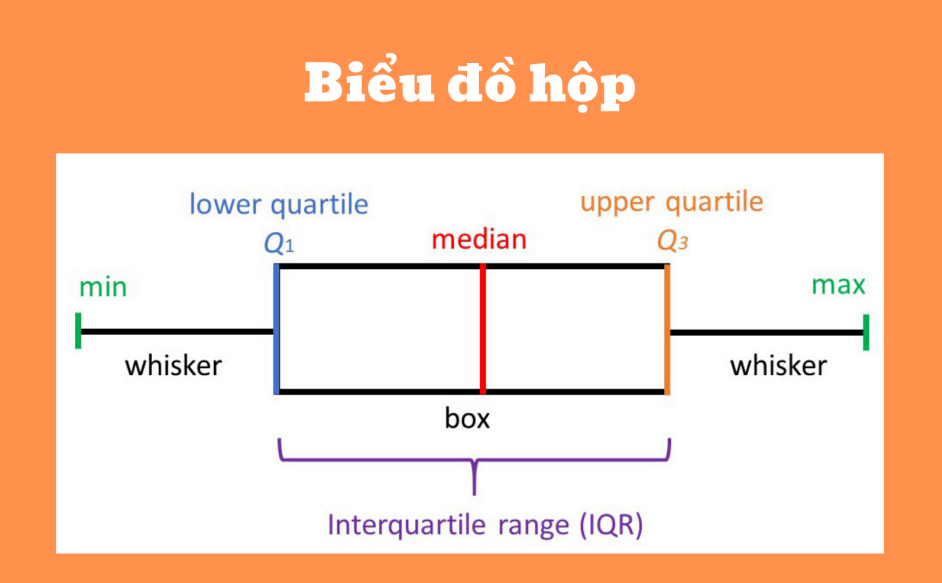
\includegraphics[width=0.8\linewidth]{2. Kiến Thức Nền/boxplot.png}
                \caption{Hình ảnh minh họa Boxplots.}
            \end{figure}
            \hspace{1pt}
            Scatterplots: Là biểu đồ dạng chấm nhằm thể hiện mối quan hệ giữa hai biến liên tục.
            \begin{figure}[H]
                \centering
                \includesvg[width=0.8\linewidth]{4. GPU/Rplot/Rplot08.svg}
                \caption{Hình ảnh minh họa Scatterplots.}
            \end{figure}

\newpage
        \subsection*{2.3 Hồi quy tuyến tính bội và phân tích phương sai ANOVA.}
        \addcontentsline{toc}{subsection}{2.3 Hồi quy tuyến tính bội và phân tích phương sai ANOVA.}
            \fontsize{13pt}{15pt}\selectfont
            \gachdau
            Hồi quy tuyến tính bội là một phương pháp được sử dụng khi ta muốn dự đoán giá trị của một biến phản hồi dựa trên giá trị của hai hoặc nhiều biến giải thích khác. Biến mà chúng ta muốn dự đoán được gọi là biến phản hồi (biến phụ thuộc). Các biến mà ta đang sử dụng để dự đoán giá trị của biến phản hồi được gọi là các biến giải thích (biến dự báo, biến phụ thuộc).\\
            \gachdau
            Hồi quy bội cũng cho phép chúng ta xác định sự phù hợp tổng thể của mô hình và đóng góp tương đối của từng yếu tố dự báo và tổng phương sai được giải thích.\\
            \gachdau
            Mô hình hồi quy tuyến tính bội liên quan đến biến Y và $p - 1$ biến dự báo X có dạng như sau:
            \vspace{-6pt}
            \begin{align*}
                Y_i = \beta_0 + \beta_1X_{i1} + \beta_2X_{i2} + ... + \beta_{p-1}X_{i(p-1)} + \epsilon_i
            \end{align*}
            \vspace{-10pt}
            \gachdau
            Hay:
            \vspace{-5pt}
            \begin{align*}
                Y_i = \beta_0 + \sum_{k=1}^{p-1}\beta_kX_{ik} + \epsilon_i
            \end{align*}
            \gachdau
            Trong đó:
            \begin{itemize}[leftmargin=3em, itemsep=-1.5em, parsep=1.6em]
                \vspace{-4pt}
                \item \fontsize{13pt}{15pt}\selectfont $Y_i$ là biến phản hồi hay biến phụ thuộc (response variable / dependent variable).
                \item \fontsize{13pt}{15pt}\selectfont $X_{ik}$ là các biến giải thích hay biến độc lập (explanatory variables / independent variables).
                \item \fontsize{13pt}{15pt}\selectfont $\beta_k$ là tham số của các biến độc lập trong đó $\beta_0$ là hệ số hồi quy (hệ số chặn).
                \item \fontsize{13pt}{15pt}\selectfont $\epsilon_i \sim N(0,\sigma^2)$ là số hạng nhiễu hay sai số ngẫu nhiên.
                \item \fontsize{13pt}{15pt}\selectfont $Y_i$ $i = 1, 2, ..., n.$
            \end{itemize}
            \vspace{-8pt}
            \gachdau
            Khi $p-1=1$ mô hình hồi quy là: $Y_i = \beta_0 + \beta_1X_{i1} + \epsilon_i$ là mô hình hồi quy tuyến tính đơn.\\
            \gachdau
            Giả định:
            \begin{itemize}[leftmargin=3em, itemsep=-1.5em, parsep=1.6em]
                \vspace{-10pt}
                \item \fontsize{13pt}{15pt}\selectfont $\epsilon_i$ có phân phổi chuẩn và phương sai không đổi.
                \item \fontsize{13pt}{15pt}\selectfont Các biến X độc lập với nhau.
            \end{itemize}
            \vspace{-8pt}
            \gachdau
            Kiểm định từng tham số hồi quy tổng thể:
            \begin{itemize}[leftmargin=3em, itemsep=-1.5em, parsep=1.6em]
                \vspace{-6pt}
                \item \fontsize{13pt}{15pt}\selectfont Trường hợp $\beta_k = 0$ thì $X_i$ và Y không có mối quan hệ nào.
                \item \fontsize{13pt}{15pt}\selectfont Trường hợp $\beta_k > 0$ thì $X_i$ và Y có mối quan hệ thuận.
                \item \fontsize{13pt}{15pt}\selectfont Trường hợp $\beta_k < 0$ thì $X_i$ và Y có mối quan hệ nghịch.
                \item \fontsize{13pt}{15pt}\selectfont Ở mức ý nghĩa $\alpha$, giả thuyết vô hiệu $H_0$ được kiểm định ở các trường hợp sau:
                \begin{enumerate}[label=(\arabic*), leftmargin=1.8em, itemsep=-1.5em, parsep=1.6em]
                    \vspace{-25pt}
                    \item \fontsize{13pt}{15pt}\selectfont $H_0: \beta_k \leq 0$ và $H_1: \beta_k > 0$
                    \item \fontsize{13pt}{15pt}\selectfont $H_0: \beta_k \geq 0$ và $H_1: \beta_k < 0$
                \end{enumerate}
                \item \fontsize{13pt}{15pt}\selectfont Giá trị kiểm định: $t = \dfrac{\beta_k}{SE(\beta_k)}$.
                \item \fontsize{13pt}{15pt}\selectfont Quyết định bác bỏ giả thuyết $H_0$:
                \begin{itemize}[leftmargin=1.5em, itemsep=-1.5em, parsep=1.6em]
                    \vspace{-22pt}
                    \item \fontsize{13pt}{15pt}\selectfont Bác bỏ giả thuyết (1) khi $t > t_{n-p,\alpha}$
                    \item \fontsize{13pt}{15pt}\selectfont Bác bỏ giả thuyết (1) khi $t < -t_{n-p,\alpha}$
                \end{itemize}
            \end{itemize}
            \vspace{-22pt}
            \gachdau
            Ma trận hồi quy:\\
            \vspace{-18pt}
            \begin{align*}
                Y = 
                \begin{bmatrix}
                    Y_1 \\
                    Y_2 \\
                    \vdots \\
                    Y_n
                \end{bmatrix},
                X = 
                \begin{bmatrix}
                    1 & x_{11} & x_{12} & \ldots & x_{1(p-1)} \\
                    1 & x_{21} & x_{22} & \ldots & x_{2(p-1)} \\
                    \vdots & \vdots & \vdots & \ddots & \vdots \\
                    1 & x_{n1} & x_{n2} & \ldots & x_{n(p-1)}
                \end{bmatrix},
                \beta = 
                \begin{bmatrix}
                    \beta_1 \\
                    \beta_2 \\
                    \vdots \\
                    \beta_n
                \end{bmatrix},
                \epsilon = 
                \begin{bmatrix}
                    \epsilon_1 \\
                    \epsilon_2 \\
                    \vdots \\
                    \epsilon_n
                \end{bmatrix}
            \end{align*}
            \gachdau
            Với dữ liệu:
            $y = 
            \begin{bmatrix}
                y_1\\
                y_2\\
                \vdots\\
                y_n
            \end{bmatrix}
            $\\
            \gachdau
            Ước tính $\beta$ bằng cực tiểu hóa:\\
            \vspace{-18pt}
            \begin{align*}
                f(\beta_0, \beta_1, \ldots, \beta{p-1} = \sum_{i=1}^{n}(y_i - (\beta_0 + \beta_1X_{i1} + \beta_2X_{i2} + ... + \beta_{p-1}X_{i(p-1)})
            \end{align*}
            \gachdau
            Khi đó: $\beta = (X^TX)^{-1}X^Ty$\\
            \gachdau
            Ý nghĩa hồi quy:
            \begin{itemize}[leftmargin=3em, itemsep=-1.5em, parsep=1.6em]
                \vspace{-8pt}
                \item \fontsize{13pt}{15pt}\selectfont $\epsilon_i$ Trường hợp: $H_0: \beta_0 = \beta_1 = \ldots = \beta_{p-1} = 0 \rightarrow Y_i = \beta_0 + \epsilon_i$, kí hiệu các dữ liệu thỏa là $y_{0i}$. Khi đó: $\overline{y} = y_{0i}$
                \item \fontsize{13pt}{15pt}\selectfont Trường hợp: $H_1:$ có ít nhất một $\beta_j \neq 0, j = 1, 2, \ldots, (p-1)$
            \end{itemize}
            \begin{table}[h]
                \centering
                \setlength{\extrarowheight}{11pt}
                \begin{tabular}{|c|c|c|c|c|}
                    \hline
                    Biến thiên & Tổng độ lệnh bình phương. & Bậc tự do & Phương sai & Giá trị kiểm định. \\
                    \hline
                    Hồi quy & SSR = $\sum_{i=1}^{n}(y_{1i} - \overline{y})^2$ & $p-1$ & MSR = $\dfrac{SSR}{p-1}$ & F = $\dfrac{MSR}{MSE}$\\
                    \hline
                    Sai số & SSE = $\sum_{i=1}^{n}(y_{i}-y_{1i})^2$ & $n-p$ & MSE = $\dfrac{SSE}{n-p}$ & \\ \hline
                    Tổng & SST = $\sum_{i=1}^{n}(y_{i}-\overline{y})^2$ & $n-1$ & & \\
                    \hline
                \end{tabular}
                \caption{Bảng ANOVA cho mô hình hồi quy tuyến tính tổng quát.}
            \end{table}
            \vspace{-13pt}
            \gachdau
            Nếu $F \leq F_{p-1,n-p,\alpha} $ chấp nhận $H_0$.\\
            \gachdau
            Nếu $F > F_{p-1,n-p,\alpha} $ bác bỏ giả thuyết $H_0$.\\
            \gachdau
            Hệ số xác định $R^2 = \dfrac{SSR}{SST} = 1 - \dfrac{SSE}{SST}$

            \hspace{1pt}
            Đại diện cho tỷ lệ biến thiên theo biến $Y_i$ với các biến dự báo $X_1i, X_2i, . . .$ Hệ số $R^2$ nói lên tính chặt chẽ giữa biến phản hồi $Y_i$ và các biến dự báo $X_ki$.\\
            \gachdau
            Ta có: $0 \leq R^2 \leq 1.$ Khi $R^2 = 0$ thì chấp nhận $H_0$. Khi $R^2 = 1$ thì tất cả các quan sát nằm trên mặt đáp ứng.\\
            \gachdau
            Nếu chúng ta bắt đầu với một mô hình hồi quy tuyến tính đơn giản với biến dự báo $X_1i$ sau đó thêm biến dự báo $X_2i$, SSE sẽ giảm (hoặc giữ nguyên) trong khi SST không đổi và do đó $R^2$ sẽ tăng (hoặc giữ nguyên). Nói cách khác, $R^2$ luôn tăng (hoặc giữ nguyên) khi có nhiều yếu tố dự báo vào mô hình hồi quy tuyến tính bội, ngay cả khi các yếu tố dự báo được thêm vào không liên quan đến biến phản hồi. Do đó bản thân $R^2$ không thể được sử dụng để giúp chúng ta xác định những yếu tố dự báo nào nên được đưa vào một mô hình và yếu tố nào nên được loại bỏ.\\
            \gachdau
            Hệ số xác định đã điều chỉnh:
            \vspace{-10pt}
            \begin{align*}
                R_\alpha^2 = \dfrac{\dfrac{SSR}{n-p}}{\dfrac{SST}{n-1}} = 1 - \big(\dfrac{n-1}{1-p})(1-R^2)
            \end{align*}


% \newpage
%     \begin{center}
%         \section*{BỘ DỮ LIỆU CPU}
%     \end{center}
%     \addcontentsline{toc}{section}{3. Bộ dữ liệu CPU}
%         \subsection*{3.1 Tiền xử lý}
%         \addcontentsline{toc}{subsection}{3.1 Tiền xử lý}
%             \subsubsection*{3.1.1 Cài đặt thư viện}
%             \addcontentsline{toc}{subsubsection}{3.1.1 Cài đặt thư viện}
%                 \gachdau
%                 Để có thể sử dụng các đoạn code được đề cập bên dưới chúng ta phải cài đặt một số thư viện sau:
% \begin{mybox}{R Code}
%     \begin{lstlisting}[language={R}]
%     install.packages("dplyr")
%     library(dplyr)
%     install.packages("2")
%     library(2)
%     install.packages("patchwork")
%     library(patchwork)
%     \end{lstlisting}
% \end{mybox}
    
%                 \gachdau
%                 Trong bài chúng tôi đã sử dụng các thư viện trên để:
%                 \begin{itemize}[leftmargin=3em, itemsep=-1.5em, parsep=1.6em]
%                     \vspace{-8pt}
%                     \item \fontsize{13pt}{15pt}\selectfont \textcolor{blue}{dplyr}: Thư viện \textcolor{blue}{dplyr} được sử dụng để thực hiện các hoạt động xử lý dữ liệu, như biến đổi dữ liệu, lọc dữ liệu, tóm tắt dữ liệu và sắp xếp dữ liệu.
%                     \item \fontsize{13pt}{15pt}\selectfont \textcolor{blue}{ggplot2}: Thư viện \textcolor{blue}{ggplot2} được sử dụng để tạo đồ thị và biểu đồ dựa trên dữ liệu.
%                     \item \fontsize{13pt}{15pt}\selectfont \textcolor{blue}{patchwork}: Thư viện \textcolor{blue}{patchwork} được sử dụng để tạo và kết hợp các đồ thị \textcolor{blue}{ggplot2} thành một đồ thị tổng thể.
%                 \end{itemize}
                
%             \subsubsection*{3.1.2 Đọc dữ liệu}
%             \addcontentsline{toc}{subsubsection}{3.1.2 Đọc dữ liệu}
%                 \gachdau
%                 Ta dùng lệnh sau để đọc dữ liệu từ file \textcolor{blue}{Intel\_CPUs.csv}
% \begin{mybox}{R Code}
%     \begin{lstlisting}[language={R}]
%     intel_cpus <- read.csv("Intel_CPUs.csv")
%     \end{lstlisting}
% \end{mybox}
%                 \gachdau
%                 Để xem 6 dòng đầu dữ liệu ta sử dụng 
% \begin{mybox}{R Code}
%     \begin{lstlisting}[language={R}]
%     head(intel_cpus)
%     \end{lstlisting}
% \end{mybox}

% \newpage
%                 \begin{figure}[H]
%                     \centering
%                     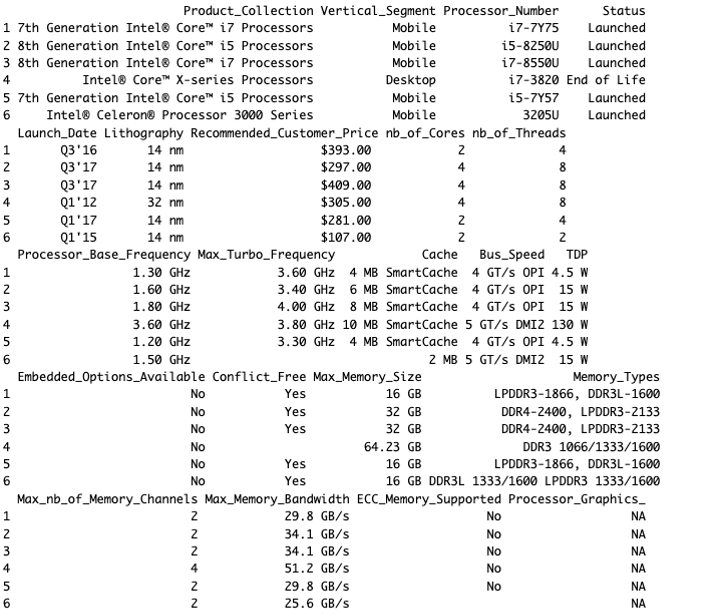
\includegraphics[width=0.49\linewidth]{3. CPU/Console/console1a.png}
%                     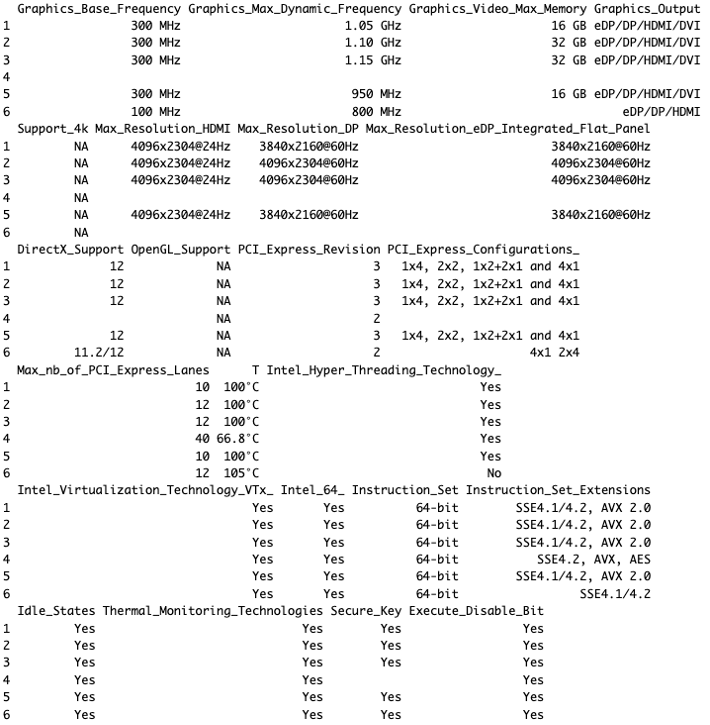
\includegraphics[width=0.42\linewidth]{3. CPU/Console/console1b.png}
%                     \caption{6 dòng đầu tiên của dữ liệu}
%                 \end{figure}

%             \subsubsection*{3.1.3 Làm sạch dữ liệu}
%             \addcontentsline{toc}{subsubsection}{3.1.3 Làm sạch dữ liệu}
%                 \gachdau
%                 Dựa trên nguồn sau có tính tham khảo tốt và phù hợp với nhu cầu sử dụng của đề tài: \href{https://www.binarytides.com/cpu-specs-explained/}{12 Important Specifications of Processor (CPU) Explained – The Ultimate Guide}. Nhóm đã thống nhất bằng cách tạo một bảng dữ liệu mới gồm những dữ liệu cần sử dụng là: \textcolor{blue}{nb\_of\_Cores}, \textcolor{blue}{nb\_of\_Threads}, \textcolor{blue}{Processor\_Base\_Frequency},	\textcolor{blue}{Max\_Turbo\_Frequency}, \textcolor{blue}{TDP}.
% \begin{mybox}{R Code}
%     \begin{lstlisting}[language={R}]
%     intel_cpus_news <- intel_cpus[, c("Recommended_Customer_Price", "nb_of_Cores","nb_of_Threads", "Processor_Base_Frequency", "Max_Turbo_Frequency", "TDP")]
%     head(intel_cpus_news)
%     \end{lstlisting}
% \end{mybox}
%                 \vspace{-17pt}
%                 \begin{figure}[H]
%                     \centering
%                     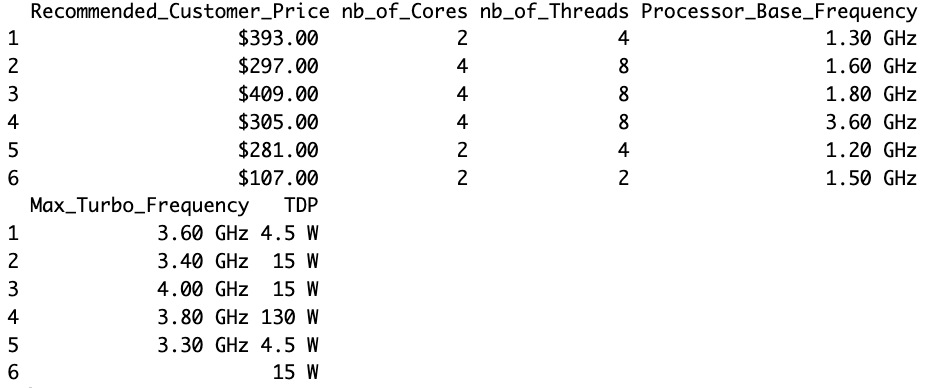
\includegraphics[width=0.7\linewidth]{3. CPU/Console/console2.png}
%                     \caption{6 dòng đầu tiên của dữ liệu sau khi lọc dữ liệu}
%                 \end{figure}

% \newpage
%                 \hspace{1pt}
%                 Lúc này dữ liệu chúng ta vẫn còn đơn vị và các các dữ liệu đang còn ở định dạng string, ta cần xóa đơn vị và chuyển về kiểu number. Trường hợp \textcolor{blue}{Recommended\_Customer\_Price} nằm giữa hai giá trị (ví dụ: \$64.00 - \$72.00), loại bỏ ký tự không phải số và tính trung bình của chúng. Chúng em còn thống nhất sử dụng đơn vị GHz cho \textcolor{blue}{Processor\_Base\_Frequency}:
% \begin{mybox}{R Code}
%     \begin{lstlisting}[language={R}]
%     intel_cpus_news <- intel_cpus_news %>%
%       mutate(
%         Recommended_Customer_Price = ifelse(
%       Recommended_Customer_Price == "N/A", 
%       NA, 
%       sapply(strsplit(Recommended_Customer_Price, " - "), function(x) {
%         price_values <- as.numeric(gsub("[^0-9.]", "", x))
%         if (!anyNA(price_values)) {
%           mean(price_values)
%         } else {
%           NA
%         }
%       })
%     ),
%     nb_of_Cores = as.numeric(gsub("[^0-9.]", "", nb_of_Cores)),
%     nb_of_Threads = as.numeric(gsub("[^0-9.]", "", nb_of_Threads)),
%     Processor_Base_Frequency = case_when(
%       grepl("GHz", Processor_Base_Frequency) ~ as.numeric(gsub("[^0-9.]", "", Processor_Base_Frequency)),
%       grepl("MHz", Processor_Base_Frequency) ~ as.numeric(gsub("[^0-9.]", "", Processor_Base_Frequency)) / 1000,
%       TRUE ~ as.numeric(Processor_Base_Frequency) # For cases with no unit specified
%     ),
%     Max_Turbo_Frequency = as.numeric(gsub("[^0-9.]", "", Max_Turbo_Frequency)),
%     TDP = as.numeric(gsub("[^0-9.]", "", TDP))
%       )
%     head(intel_cpus_news)
%     \end{lstlisting}
% \end{mybox}

% \newpage
%                 \begin{figure}[H]
%                     \centering
%                     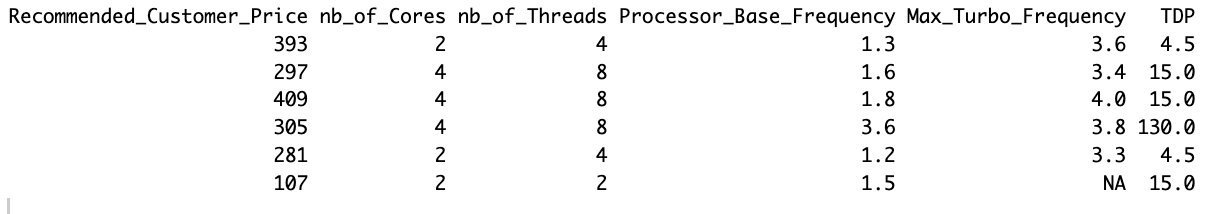
\includegraphics[width=0.8\linewidth]{3. CPU/Console/console3.png}
%                     \caption{6 dòng đầu tiên của dữ liệu sau khi dữ liệu sau khi chuyển thành dạng số}
%                 \end{figure}
%                 \vspace{-10pt}
%                 \gachdau
%                 Sau khi hoàn tất dữ liệu ta thống kê số dữ liệu bị khuất của từng biến:
% \begin{mybox}{R Code}
%     \begin{lstlisting}[language={R}]
%     missing_counts <- colSums(is.na(intel_cpus_news))
%     missing_counts
%     \end{lstlisting}
% \end{mybox}
%                 \vspace{-17pt}
%                 \begin{figure}[H]
%                     \centering
%                     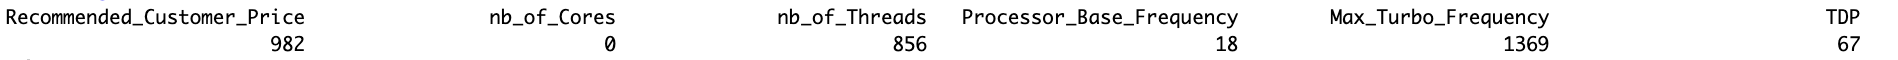
\includegraphics[width=0.8\linewidth]{3. CPU/Console/console4.png}
%                     \caption{Thống kê dữ liệu bị khuyết ở các cột}
%                 \end{figure}
%                 \vspace{-10pt}
%                 \gachdau
%                 Quan sát bảng thống kê ta thấy được như sau:
%                 \begin{itemize}[leftmargin=3.5em, itemsep=-1.5em, parsep=1.6em]
%                     \vspace{-6pt}
%                     \item \fontsize{13pt}{15pt}\selectfont 982 dữ liệu thuộc biến \textcolor{blue}{Recommended\_Customer\_Price} bị khuyết.
%                     \item \fontsize{13pt}{15pt}\selectfont 0 dữ liệu thuộc biến \textcolor{blue}{nb\_of\_Cores} bị khuyết.
%                     \item \fontsize{13pt}{15pt}\selectfont 856 dữ liệu thuộc biến \textcolor{blue}{nb\_of\_Threads} bị khuyết.
%                     \item \fontsize{13pt}{15pt}\selectfont 18 dữ liệu thuộc biến \textcolor{blue}{Processor\_Base\_Frequency} bị khuyết.
%                     \item \fontsize{13pt}{15pt}\selectfont 1369 dữ liệu thuộc biến \textcolor{blue}{Max\_Turbo\_Frequency} bị khuyết.
%                     \item \fontsize{13pt}{15pt}\selectfont 67 dữ liệu thuộc biến \textcolor{blue}{TDP} bị khuyết.
%                 \end{itemize}
%                 \vspace{-8pt}
%                 \gachdau
%                 Từ đó nhóm chúng tôi đã đưa ra một số phương pháp xử lí dữ liệu bị khuyết:
%                 \begin{itemize}[leftmargin=3.5em, itemsep=-1.5em, parsep=1.6em]
%                     \vspace{-6pt}
%                     \item \fontsize{13pt}{15pt}\selectfont Ngoài biến \textcolor{blue}{Recommended\_Customer\_Price} là yếu tố chính để dự đoán số liệu trong đề tài này, tất cả các dữ liệu khuyết của các biến còn lại sẽ được thay thế bằng giá trị trung bình tương ứng với từng biến.
%                     \item \fontsize{13pt}{15pt}\selectfont Vì số lượng dữ liệu khuyết của biến \textcolor{blue}{Max\_Turbo\_Frequency} chiếm hơn 50\% tổng số dữ liệu của biến nên nhóm xin đề xuất loại bỏ biến này để không gây ảnh hưởng đến dữ liệu chung.
%                 \end{itemize}
%                 \gachdau
%                 Qua đó nhóm sẽ lọc lại dữ liệu bằng cách:
%                 \begin{itemize}[leftmargin=3.5em, itemsep=-1.5em, parsep=1.6em] 
%                     \vspace{-7pt}
%                     \item \fontsize{13pt}{15pt}\selectfont Xóa dữ liệu thuộc biến \textcolor{blue}{Max\_Turbo\_Frequency}
% \begin{mybox}{R Code}
%     \begin{lstlisting}[language={R}] 
%     intel_cpus_news <- intel_cpus_news[, -5]
%     \end{lstlisting}
% \end{mybox}

% \newpage
%                     \item \fontsize{13pt}{15pt}\selectfont Thay thế các giá trị NA bằng các giá trị trung bình sau đó lọc và bỏ các dòng chứa dữ liệu bị khiếm khuyết của biến \textcolor{blue}{Recommended\_Customer\_Price}.
% \begin{mybox}{R Code}
%     \begin{lstlisting}[language={R}] 
%     %%Tim gia tri trung binh cua cac bien
%     mean_values <- sapply(intel_cpus_news[, -1], function(x) mean(x, na.rm = TRUE))
%     mean_values
%     %%Cac du lieu khuyet cua cac bien con lai se duoc thay the bang gia tri trung binh tuong ung voi cac bien
%     intel_cpus_news <- intel_cpus_news %>%
%   mutate(
%     Recommended_Customer_Price = ifelse(is.na(Recommended_Customer_Price), mean_values["Recommended_Customer_Price"], Recommended_Customer_Price),
%     nb_of_Cores = ifelse(is.na(nb_of_Cores), mean_values["nb_of_Cores"], nb_of_Cores),
%     nb_of_Threads = ifelse(is.na(nb_of_Threads), mean_values["nb_of_Threads"], nb_of_Threads),
%     Processor_Base_Frequency = ifelse(is.na(Processor_Base_Frequency), mean_values["Processor_Base_Frequency"], Processor_Base_Frequency),
%     TDP = ifelse(is.na(TDP), mean_values["TDP"], TDP)
%   )

% head(intel_cpus_news)
%     %%Loc lay du lieu khong bi khiem khuyet cua Release_Price
%     intel_cpus_news_clean <- na.omit(intel_cpus_news)
%     head(intel_cpus_news_clean)
%     \end{lstlisting}
% \end{mybox}

%                     \begin{figure}[H]
%                         \centering
%                         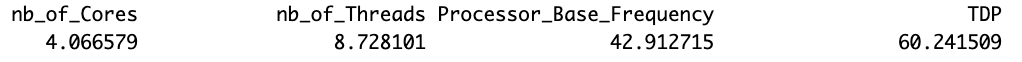
\includegraphics[width=0.8\linewidth]{3. CPU/Console/console5.png}
%                         \caption{Thống kê dữ liệu bị khuyết ở các cột}
%                     \end{figure}
%                     \item \fontsize{13pt}{15pt}\selectfont Xóa dữ các dòng bị khuyết của biến \textcolor{blue}{Recommended\_Customer\_Price}.
% \newpage
% \begin{mybox}{R Code}
%     \begin{lstlisting}[language={R}] 
%     intel_cpus_news_clean <- na.omit(intel_cpus_news)
%     head(intel_cpus_news_clean)
%     \end{lstlisting}
% \end{mybox}

%                     \begin{figure}[H]
%                         \centering
%                         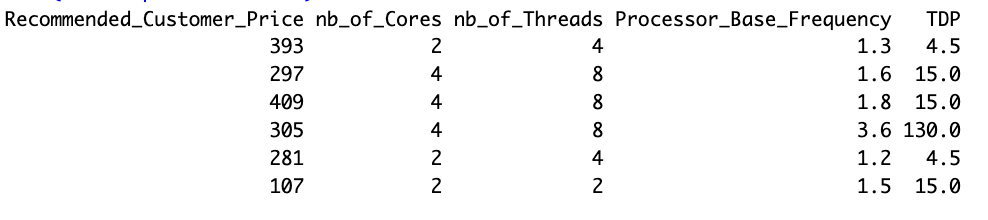
\includegraphics[width=0.8\linewidth]{3. CPU/Console/console6.png}
%                         \caption{Dữ liệu sau khi lọc bỏ các hàng bị khuyết của biến \textcolor{blue}{Recommended\_Customer\_Price}}
%                     \end{figure}
%                     \vspace{-18pt}
%                     \item \fontsize{13pt}{15pt}\selectfont Đánh lại số thứ tự các dòng dữ liệu.
% \begin{mybox}{R Code}
%     \begin{lstlisting}[language={R}] 
%     rownames(intel_cpus_news_clean) <- NULL
%     head(intel_cpus_news_clean)
%     \end{lstlisting}
% \end{mybox}
%                     \begin{figure}[H]
%                         \centering
%                         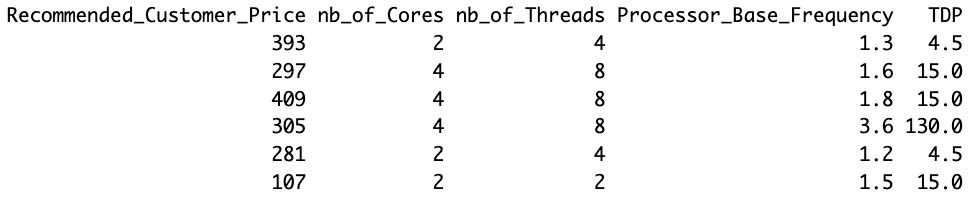
\includegraphics[width=0.8\linewidth]{3. CPU/Console/console7.png}
%                         \caption{Dữ liệu sau khi đánh lại số thứ tự}
%                     \end{figure}
%                 \end{itemize}
                
%         \vspace{-1.2cm}       
%         \subsection*{3.2 Thống kê tả}
%         \addcontentsline{toc}{subsection}{3.2 Thống kê tả}
%             \subsubsection*{3.2.1 Scatter plots}
%             \addcontentsline{toc}{subsubsection}{3.2.1 Scatter plots}
%                 \vspace{-10pt}
%                 \begin{figure}[H]
%                     \centering
%                     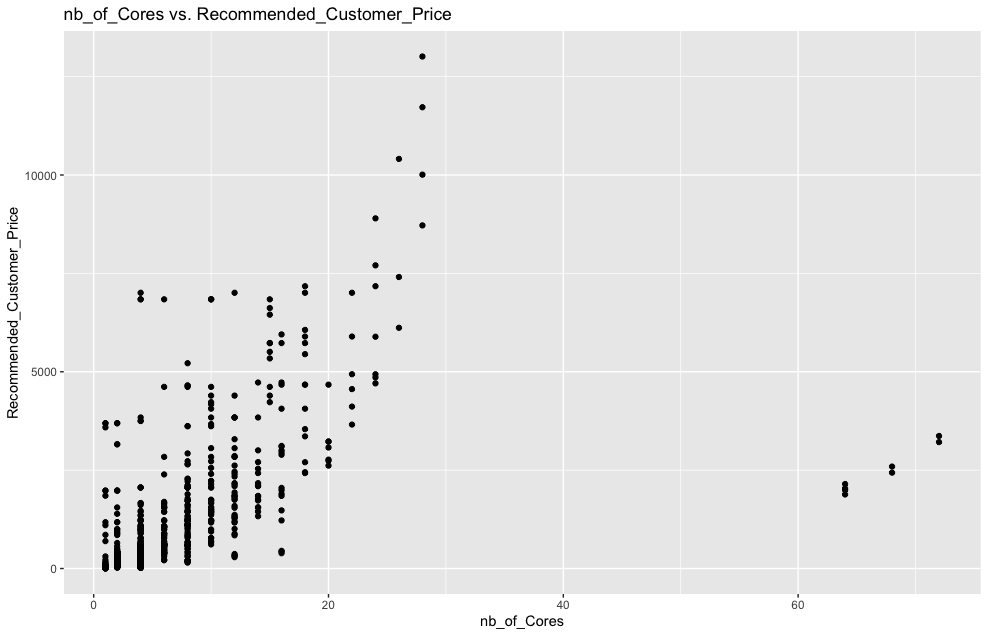
\includegraphics[width=0.47\textwidth]{3. CPU/Rplot/Rplot01.png}
%                     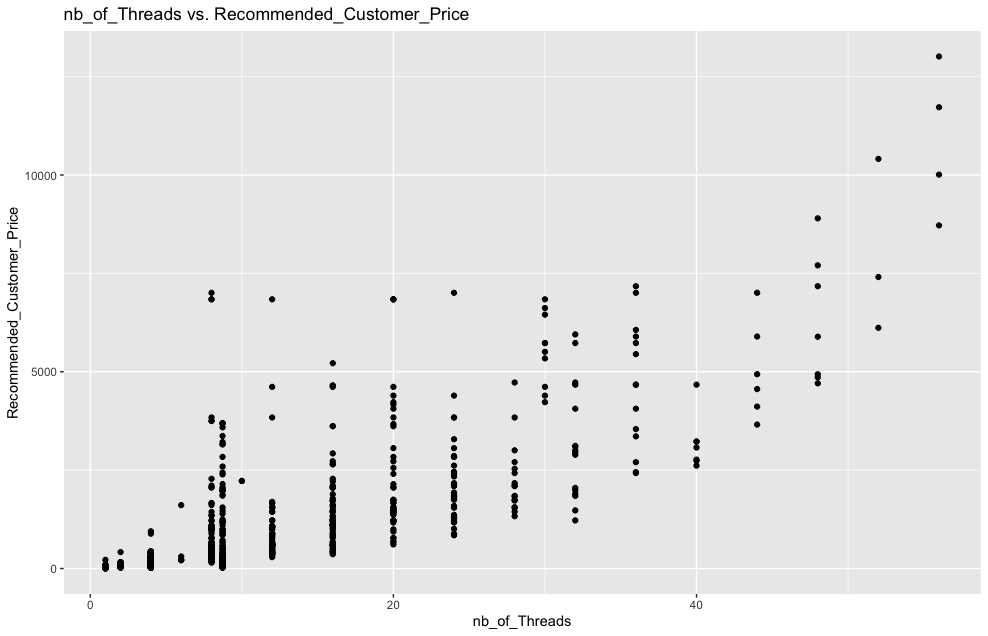
\includegraphics[width=0.47\textwidth]{3. CPU/Rplot/Rplot02.png}
%                 \end{figure}
% \newpage
%                 \begin{figure}[H]
%                     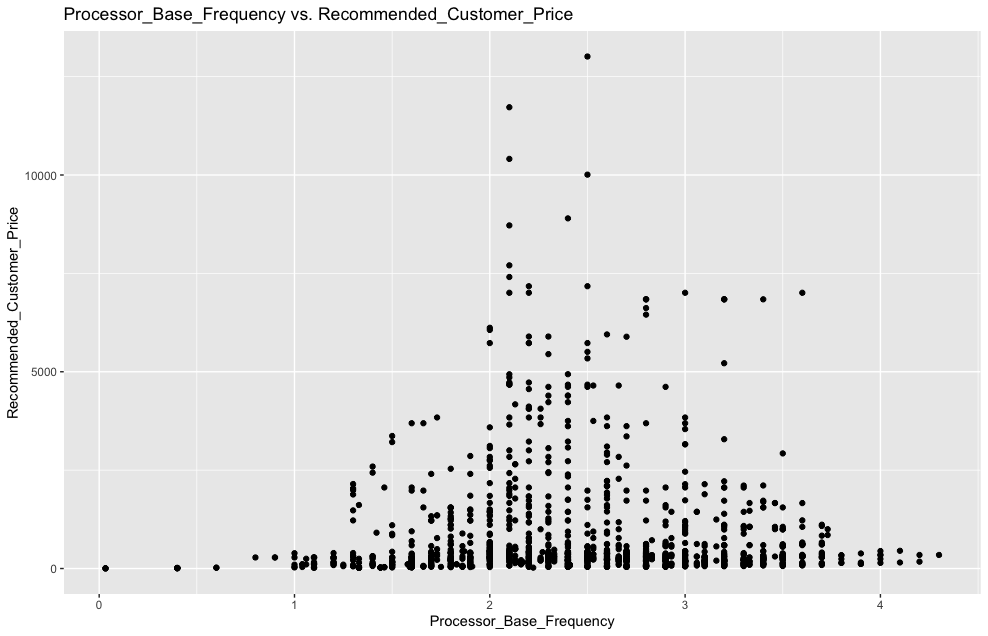
\includegraphics[width=0.47\textwidth]{3. CPU/Rplot/Rplot03.png}
%                     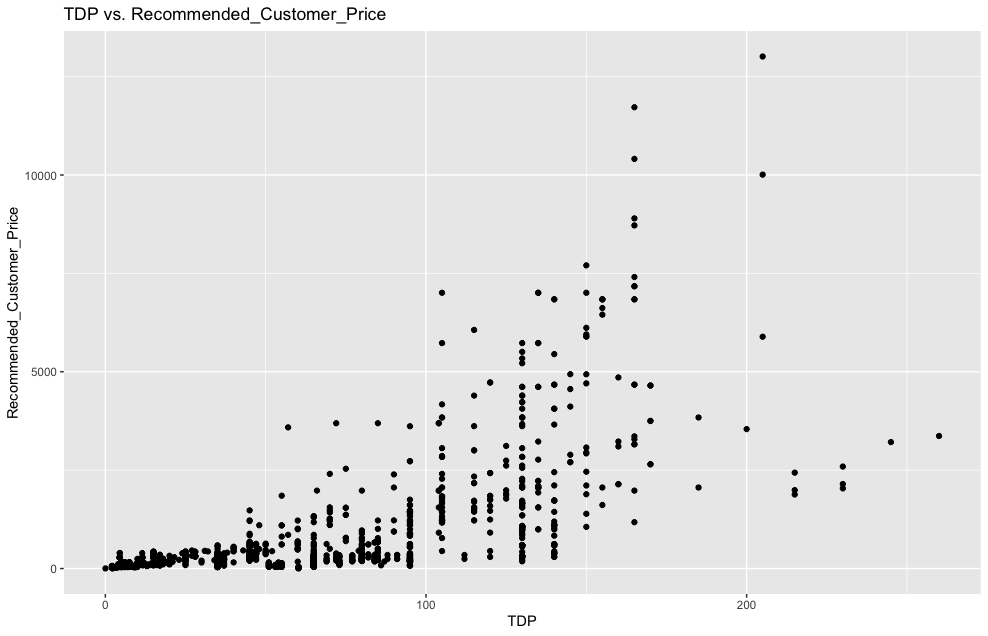
\includegraphics[width=0.47\textwidth]{3. CPU/Rplot/Rplot04.png}
%                     \caption{Biểu đồ phân tán của 4 biến đối với biến \textcolor{blue}{Recommended\_Customer\_Price}}
%                 \end{figure}
%                 \vspace{-16pt}
%                 \gachdau
%                 \fontsize{13pt}{15pt}\selectfont \textbf{Nhận xét}: Giá bán lẻ khuyến nghị của khách hàng có xu hướng tăng cùng với tần số cơ sở của bộ xử lý. Mối tương quan này được thể hiện bằng một đường thẳng có độ dốc dương.

%             \subsubsection*{3.2.2 Histogram}
%             \addcontentsline{toc}{subsubsection}{3.2.2 Histogram}
%                 \vspace{-15pt}
%                 \begin{figure}[H]
%                     \centering
%                     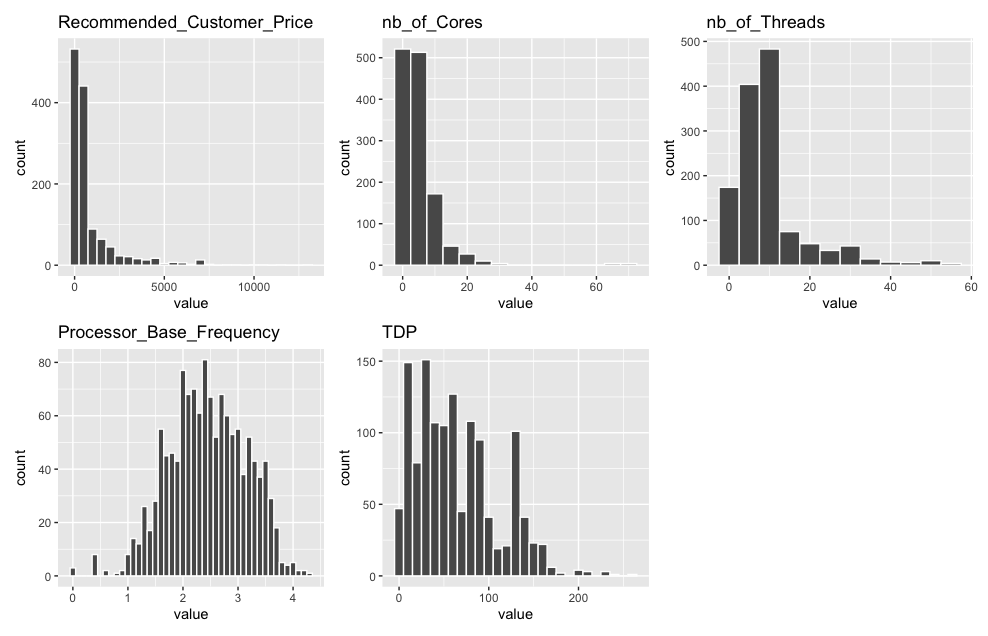
\includegraphics[width=0.9\linewidth]{3. CPU/Rplot/Rplot05.png}
%                     \caption{Biểu đồ cột của 5 biến}
%                 \end{figure}
%                 \vspace{-15pt}
%                 \gachdau
%                 \fontsize{13pt}{15pt}\selectfont \textbf{Nhận xét}: Dựa trên các Histogram, ta có thể thấy rằng giá trị của biến “\textcolor{blue}{Recommended\_Customer\_Price}” chủ yếu giao động ở mức 0\$ đến 1000\$ và tập trung chủ yếu trong khoảng 0\$ đến 500\$.

% \newpage
%             \subsubsection*{3.2.3 Boxplot}
%             \addcontentsline{toc}{subsubsection}{3.2.3 Boxplot}
%                 \vspace{-15pt}
%                 \begin{figure}[H]
%                     \centering
%                     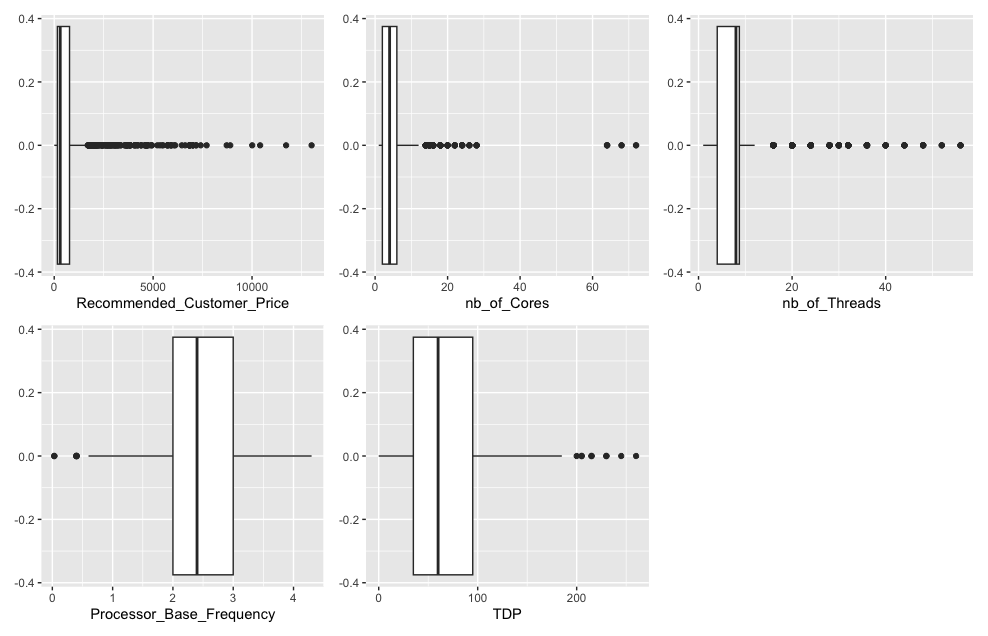
\includegraphics[width=0.7\linewidth]{3. CPU/Rplot/Rplot06.png}
%                     \caption{Biểu đồ cột của 5 biến}
%                 \end{figure}
%                 \vspace{-15pt}
%                 \gachdau
%                 \fontsize{13pt}{15pt}\selectfont \textbf{Nhận xét}: Giá bán lẻ khuyến nghị của khách hàng có trung vị là 10.000 USD. Tần số cơ sở của bộ xử lý có trung vị là 2.000 MHz. Râu trên của biểu đồ hộp cho thấy có một số bộ xử lý có giá bán lẻ khuyến nghị cao hơn 12.000 USD, mặc dù chúng có tần số cơ sở thấp hơn mức trung bình. Râu dưới của biểu đồ hộp cho thấy có một số bộ xử lý có giá bán lẻ khuyến nghị thấp hơn 8.000 USD, mặc dù chúng có tần số cơ sở cao hơn mức trung bình.

%         \subsection*{3.3 Xây dựng mô hình hồi quy tuyến tính}
%         \addcontentsline{toc}{subsection}{3.3 Xây dựng mô hình hồi quy tuyến tính}
%             \gachdau
%             Với bộ dữ liệu trên, nhóm muốn tìm hiểu những nhân tố nào có ảnh hưởng và ảnh hưởng như thế nào đến giá bán CPU.\\
%             \gachdau
%             Xét mô hình hổi quy gồm:
%             \begin{itemize}[leftmargin=3.5em, itemsep=-1.5em, parsep=1.6em]
%                 \vspace{-6pt}
%                 \item \fontsize{13pt}{15pt}\selectfont Biến phụ thuộc: \textcolor{blue}{Recommended\_Customer\_Price}
%                 \item \fontsize{13pt}{15pt}\selectfont Biến độc lập: \textcolor{blue}{nb\_of\_Cores}, \textcolor{blue}{nb\_of\_Threads}, \textcolor{blue}{Processor\_Base\_Frequency}, \textcolor{blue}{TDP}.
%             \end{itemize}
%             \gachdau
%             Ta có mô hình được biểu diễn như sau:
%             \begin{align*}
%                 Recommended\_Customer\_Price = \beta_0 + \beta_1 \cdot nb\_of\_Cores + \beta_2 \cdot nb\_of\_Threads\\
%                 + \beta_3 \cdot Processcor\_Base\_Frequency + \beta_4 \cdot TDP
%             \end{align*}
%             \gachdau
%             Kiểm định các hệ số hồi quy:
%             \begin{itemize}[leftmargin=3.5em, itemsep=-1.5em, parsep=1.6em]
%                 \vspace{-6pt}
%                 \item \fontsize{13pt}{15pt}\selectfont Giả thuyết $H_0$: Hệ số hồi quy không có ý nghĩa thống kê $(\beta_i = 0)$
%                 \item \fontsize{13pt}{15pt}\selectfont Giả thuyết $H_1$: Hệ số hồi quy có ý nghĩa thống kê $(\beta_i \neq 0)$
%             \end{itemize}

% \newpage
%             \begin{figure}[H]
%                 \centering
%                 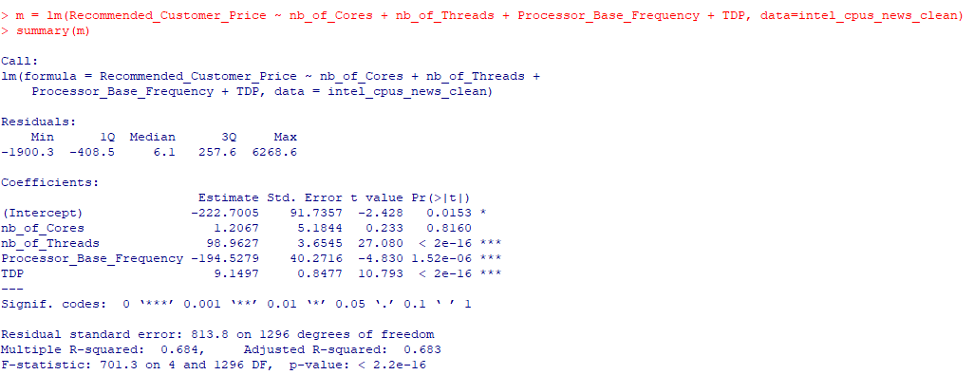
\includegraphics[width=0.8\linewidth]{3. CPU/Thống kê suy diễn/Ước lượng hệ số.png}
%                 \caption{Ước lượng hệ số $\beta_i$ $(0 \leq i \leq 4)$ dựa trên tệp intel\_cpus\_news}
%             \end{figure}
%             \vspace{-15pt}
%             \gachdau
%             Từ kết quả, ta thu được:
%             \vspace{-5pt}
%             \begin{align*}
%                 \beta_0 = -222.7005; \beta_1 = 1.2067; \beta_2 = 98.9627; \beta_3 = -194.5279; \beta_4 = 9.1497
%             \end{align*}
%             \gachdau
%             Do $P_r (> |t|)$ của tất cả các biến trừ nb\_of\_Cores và hệ số tự do đều bé hơn mức ý nghĩa 0.05, nên ta bác bỏ giả thuyết $H_0$. Do đó hệ số ứng với các biến này đều có ý nghĩa đối với mô hình hồi quy mà ta đã xây dựng.\\
%             \gachdau
%             Như vậy đường thẳng hồi quy ước lượng được cho bởi phương trình:
%             \begin{align*}
%                 Recommended\_Customer\_Price = 98.9627 \cdot nb\_of\_Threads -\\
%                 194.5279 \cdot Processcor\_Base\_Frequency + 9.1497 \cdot TDP
%             \end{align*}
%             \gachdau
%             Ngoài ra ta cũng thấy được hệ số $R^2$ hiệu chỉnh là 0.683 cho thấy đến 68.30\% sự biến thiên trong giá máy tính được giải thích bằng các biến độc lập, 31.70\% còn lại có thể do sai số hoặc các biến độc lập khác chưa được đưa vào mô hình.\\
%             \gachdau
%             Cuối cùng, ta đi kiểm tra tính phù hợp của mô hình vừa thu được thông qua các đồ thị:
%             \begin{itemize}[leftmargin=3.5em, itemsep=-1.5em, parsep=1.6em]
%                 \vspace{-6pt}
%                 \item \fontsize{13pt}{15pt}\selectfont Giả thiết 1: Dữ liệu có tính tuyến tính, quan hệ giữa biến phụ thuộc và các biến độc lập để dự báo là tuyến tính.
%                 \item \fontsize{13pt}{15pt}\selectfont Giả thiết 2: Sai số có kỳ vọng bằng 0.
%                 \item \fontsize{13pt}{15pt}\selectfont Giả thiết 3: Sai số ngẫu nhiên có phân phối chuẩn
%                 \item \fontsize{13pt}{15pt}\selectfont Giả thiết 4: Phương sai của sai số ngẫu nhiên không đổi.
%                 \item \fontsize{13pt}{15pt}\selectfont Giả thiết 5: Sai số là độc lập với nhau.
%             \end{itemize}
%             \vspace{-5pt}
%             \begin{figure}[H]
%                     \centering
%                     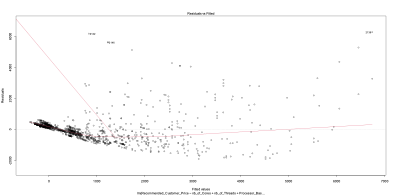
\includegraphics[width=0.49\textwidth]{3. CPU/Thống kê suy diễn/Rplot1.png}
%                     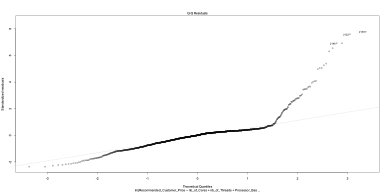
\includegraphics[width=0.49\textwidth]{3. CPU/Thống kê suy diễn/Rplot2.png}
%                 \end{figure}
% \newpage
%             \begin{figure}[H]
%                 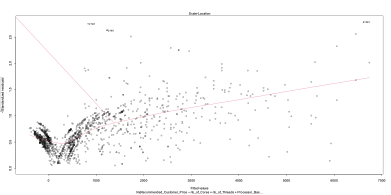
\includegraphics[width=0.49\textwidth]{3. CPU/Thống kê suy diễn/Rplot3.png}
%                 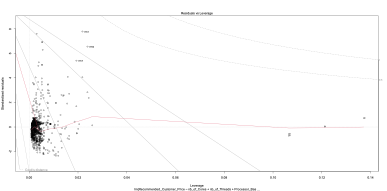
\includegraphics[width=0.49\textwidth]{3. CPU/Thống kê suy diễn/Rplot4.png}
%             \end{figure}
%             \gachdau
%             \fontsize{13pt}{15pt}\selectfont \textbf{Nhận xét}: \begin{itemize}[leftmargin=3.5em, itemsep=-1.5em, parsep=1.6em]
%                 \vspace{-6pt}
%                 \item \fontsize{13pt}{15pt}\selectfont Đồ thị thứ 1 (Residuals vs Fitted) vẽ các giá trị sai số so với dự báo, dùng để kiểm tra giả thiết tuyến tính của dữ liệu và giả thiết sai số có kỳ vọng bằng 0. Đường màu đỏ là đường cong, không trùng với đường nằm ngang cho thấy giả thiết tính của dữ liệu chưa được thỏa mãn và sai số có kỳ vọng bằng 0 chưa được thỏa mãn.
%                 \item \fontsize{13pt}{15pt}\selectfont Đồ thị thứ 2 (Q-Q Residuals) vẽ sai số được chuẩn hóa, dùng để kiểm tra giả thiết sai số có phân phối chuẩn. Vì đồ thị trên có nhiều điểm sai số lệch khỏi đường phân phối chuẩn nên giả thiết sai số có phân phối chuẩn chưa được thỏa mãn.
%                 \item \fontsize{13pt}{15pt}\selectfont Đồ thị thứ 3 (Scale – Location) vẽ căn bậc hai của sai số được chuẩn hóa dùng để kiểm tra giả định phương sai của sai số là hằng số. Các điểm phân tán một cách ngẫu nhiên, không tập trung nhiều quanh đường màu đỏ nên giả định về phương sai của sai số là hằng số được thỏa mãn.
%                 \item \fontsize{13pt}{15pt}\selectfont Đồ thị thứ 4 (Residuals vs Leverage) dùng để xác định các điểm có ảnh hưởng cao. Các điểm đó là 1157, 1159 và 1161.
%                 \item \fontsize{13pt}{15pt}\selectfont Mô hình dự báo khá chính xác giá CPU khi dưới 1000, các điểm sai số nằm gần đường thẳng nằm ngang $y = 0$. Từ đó cho thấy mô hình trên là khá phù hợp. 
%             \end{itemize}
%               \gachdau
%             \fontsize{13pt}{15pt}\selectfont \textbf{Dự báo cho giá CPU:}:
%             \begin{itemize}[leftmargin=3.5em, itemsep=-1.5em, parsep=1.6em]
%                 \vspace{-6pt}
%                 \item \fontsize{13pt}{15pt}\selectfont Dựa trên mô hình hồi quy đã xây dựng, thử dự báo giá một CPU có 4 nhân, 8 luồng, tần số cơ bản 1.60GHz và công suất thoát nhiệt cơ bản 15W.
%                 \begin{figure}[H]
%                     \centering
%                     \includegraphics[width=0.8\linewidth]{3. CPU/Thống kê suy diễn/Dự báo giá.png}
%                 \end{figure}
%                 \item \fontsize{13pt}{15pt}\selectfont Giá dự báo 339.8282 với khoảng tin cậy so với giá trị dự báo (320.3875, 479.2689).
%             \end{itemize}

\newpage
    \begin{center}
        \section*{TIỀN XỬ LÝ GPU}
    \end{center}
    \addcontentsline{toc}{section}{3. Tiền xử lý GPU}
        \subsection*{3.1 Cài đặt thư viện}
        \addcontentsline{toc}{subsection}{3.1 Cài đặt thư viện}
            \gachdau
            Để có thể sử dụng các đoạn code được đề cập bên dưới chúng ta phải cài đặt một số thư viện sau:
\begin{mybox}{R Code}
    \begin{lstlisting}[language={R}]
    install.packages("dplyr")
    library(dplyr)
    install.packages("ggplot2")
    library(ggplot2)
    install.packages("patchwork")
    library(patchwork)
    \end{lstlisting}
\end{mybox}
            \hspace{1pt}
            Trong bài chúng tôi đã sử dụng các thư viện trên để:
            \begin{itemize}[leftmargin=3em, itemsep=-0.15em]
                \vspace{-6pt}
                \item \fontsize{13pt}{15pt}\selectfont \textcolor{blue}{dplyr}: Thư viện \textcolor{blue}{dplyr} được sử dụng để thực hiện các hoạt động xử lý dữ liệu, như biến đổi dữ liệu, lọc dữ liệu, tóm tắt dữ liệu và sắp xếp dữ liệu.
                \item \fontsize{13pt}{15pt}\selectfont \textcolor{blue}{ggplot2}: Thư viện \textcolor{blue}{ggplot2} được sử dụng để tạo đồ thị và biểu đồ dựa trên dữ liệu.
                \item \fontsize{13pt}{15pt}\selectfont \textcolor{blue}{patchwork}: Thư viện \textcolor{blue}{patchwork} được sử dụng để tạo và kết hợp các đồ thị \textcolor{blue}{ggplot2} thành một đồ thị tổng thể.
            \end{itemize}
                
        \subsection*{3.2 Đọc dữ liệu}
        \addcontentsline{toc}{subsection}{3.2 Đọc dữ liệu}
            \gachdau
            Ta dùng lệnh sau để đọc dữ liệu từ file \textcolor{blue}{All\_GPU.csv} và để xem 10 dòng dữ liệu đầu tiên.
\begin{mybox}{R Code}
    \begin{lstlisting}[language={R}]
    all_gpus <- read.csv("ALL_GPUs.csv")
    head(all_gpus,10)
    \end{lstlisting}
\end{mybox}

\newpage
            \begin{figure}[H]
                \vspace{-16pt}
                \centering
                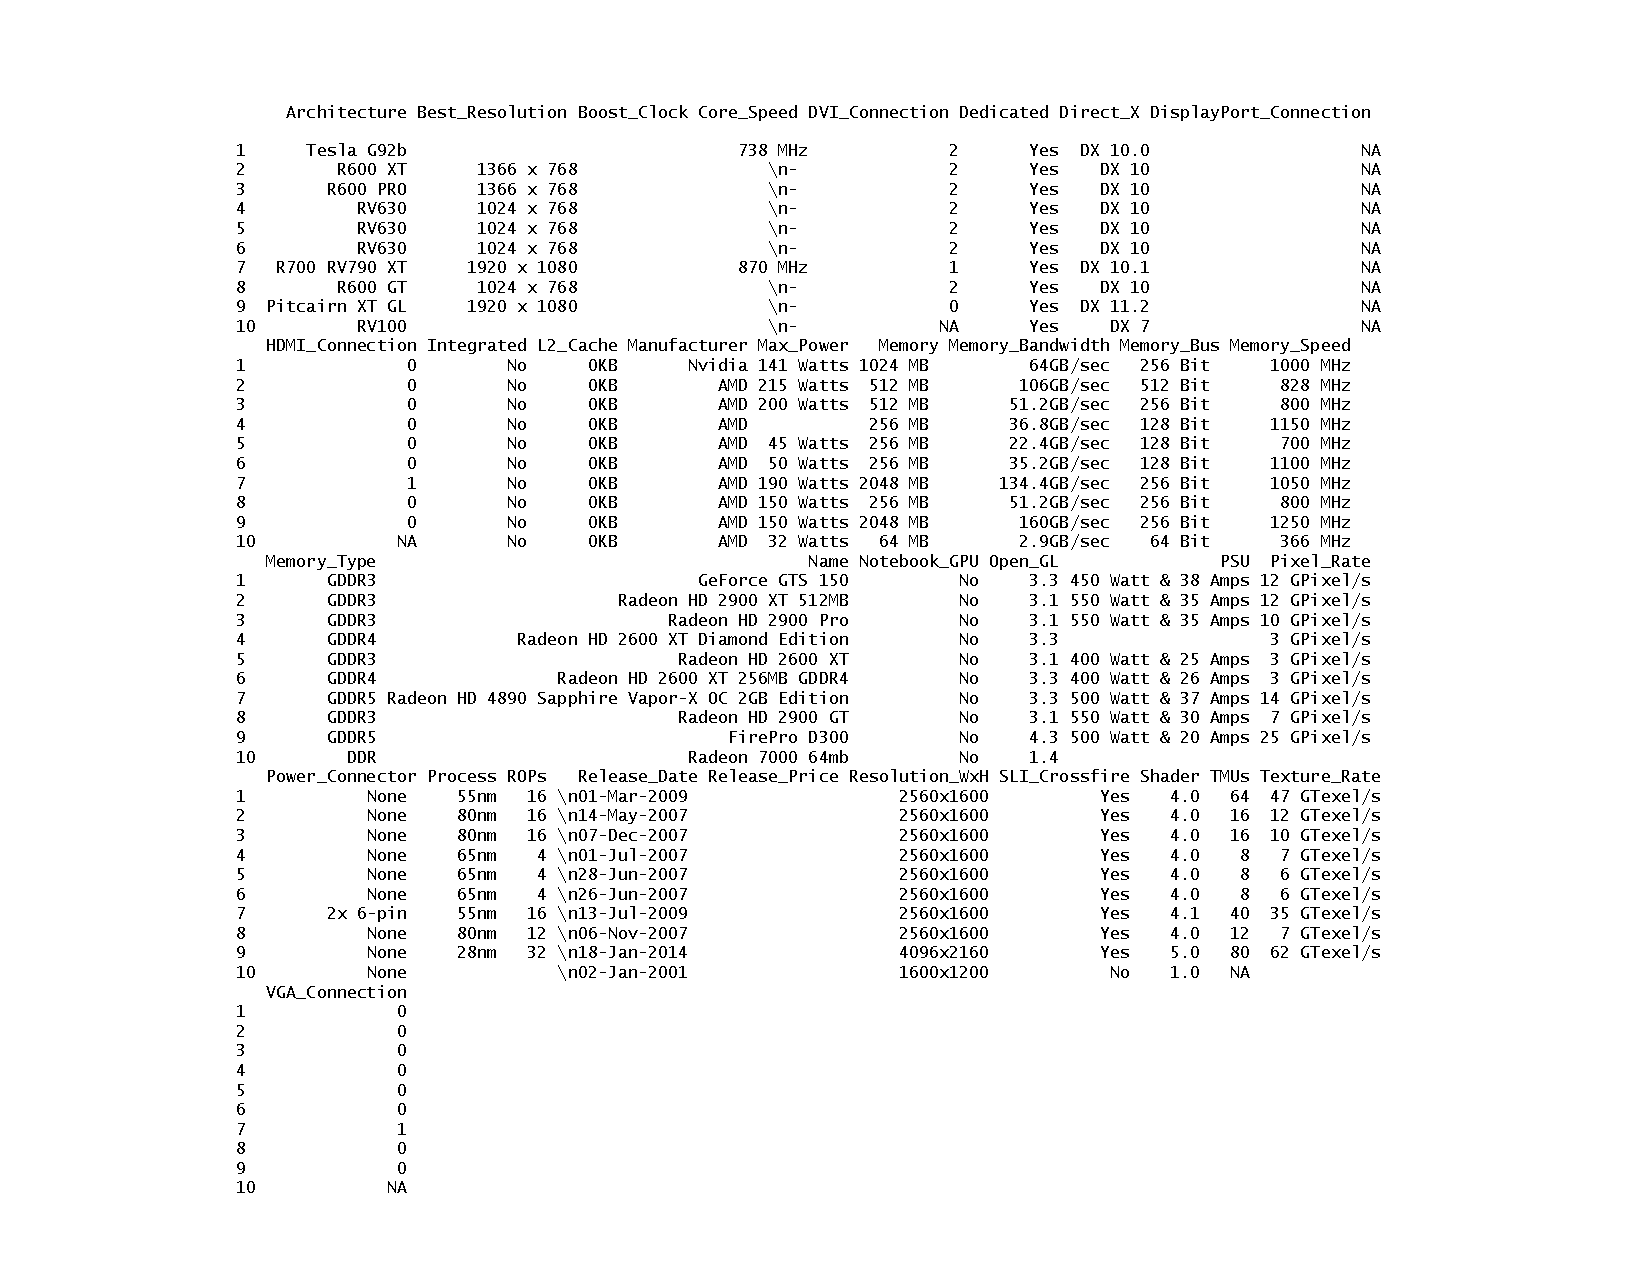
\includegraphics[width=0.94\textwidth]{4. GPU/Console/console1.pdf}
                \caption{10 dòng đầu tiên của dữ liệu}
            \end{figure}          
       
        \subsection*{3.3 Làm sạch dữ liệu}
        \addcontentsline{toc}{subsection}{3.3 Làm sạch dữ liệu}
            \gachdau
            Dựa trên nguồn sau có tính tham khảo tốt và phù hợp với nhu cầu sử dụng của đề tài: \href{https://hoanghapc.vn/card-man-hinh-va-cac-thong-so-quan-trong-thuong-gap}{Card màn hình (VGA) và các thông số quan trọng thường gặp}. Nhóm đã thống nhất bằng cách tạo một bảng dữ liệu mới gồm những dữ liệu cần sử dụng là: \textcolor{blue}{Max\_Power}, \textcolor{blue}{Boost\_Clock}, \textcolor{blue}{Core\_Speed}, \textcolor{blue}{Memory}, \textcolor{blue}{Memory\_Bandwidth}, \textcolor{blue}{Memory\_Bus}, \textcolor{blue}{Memory\_Speed}, \textcolor{blue}{Release\_Price}, \textcolor{blue}{Texture\_Rate}
\begin{mybox}{R Code}
    \begin{lstlisting}[language={R}]
    all_gpus_news <- all_gpus[, c("Max_Power","Boost_Clock", "Core_Speed", "Memory", "Memory_Bandwidth", "Memory_Bus", "Memory_Speed", "Release_Price", "Texture_Rate")]
    head(all_gpus_news, n=10)
    \end{lstlisting}
\end{mybox}

\newpage
            \begin{figure}[H]
                \centering
                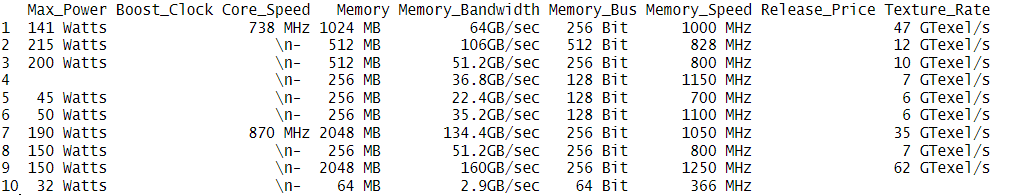
\includegraphics[width=\linewidth]{4. GPU/Console/console2.png}
                \caption{10 dòng đầu tiên của dữ liệu sau khi lọc dữ liệu}
            \end{figure}
            \vspace{-16pt}
            \hspace{1pt}
            Lúc này dữ liệu chúng ta vẫn còn đơn vị và các các dữ liệu đang còn ở định dạng string, ta cần xóa đơn vị và chuyển về kiểu number:

\begin{mybox}{R Code}
\begin{lstlisting}[language={R}]
 all_gpus_news <- all_gpus_news %>%
 mutate(
   Max_Power = as.numeric(gsub("[^0-9.]","", Max_Power)),
   Boost_Clock = as.numeric(gsub("[^0-9.]", "", Boost_Clock)),
   Core_Speed = as.numeric(gsub("[^0-9.]","", Core_Speed)),
   Memory = as.numeric(gsub("[^0-9.]","", Memory)),
   Memory_Bandwidth = as.numeric(gsub("[^0-9.]", "", Memory_Bandwidth)),
   Memory_Bus = as.numeric(gsub("[^0-9.]", "", Memory_Bus)),
   Memory_Speed = as.numeric(gsub("[^0-9.]", "", Memory_Speed)),
   Release_Price = as.numeric(gsub("[^0-9.]", "", Release_Price)),
   Texture_Rate = as.numeric(gsub("[^0-9.]", "", Texture_Rate))
  )
  head(all_gpus_news,n = 10)
\end{lstlisting}
\end{mybox}

\newpage
            \begin{figure}[H]
                \centering
                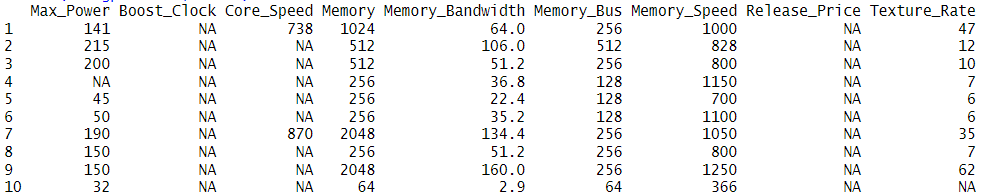
\includegraphics[width=0.7\linewidth]{4. GPU/Console/console3.png}
                \caption{10 dòng đầu tiên của dữ liệu sau khi dữ liệu chuyển thành dạng số}
            \end{figure}
            \vspace{-18pt}
            \hspace{1pt}
            Sau khi hoàn tất dữ liệu ta thống kê số dữ liệu bị khuất của từng biến:
\begin{mybox}{R Code}
    \begin{lstlisting}[language={R}]
    missing_counts <- colSums(is.na(all_gpus_news))
    missing_counts
    \end{lstlisting}
\end{mybox}
            \vspace{-10pt}
            \begin{figure}[!h]
                \vspace{-4pt}
                \centering
                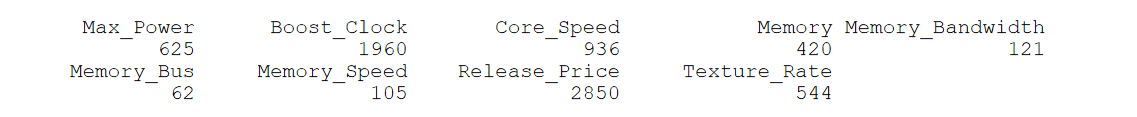
\includegraphics[width=0.8\linewidth]{4. GPU/Console/console4.png}
                \caption{Thống kê dữ liệu bị khuyết ở các cột}
            \end{figure}
            \vspace{-16pt}
            \hspace{1pt}
            Quan sát bảng thống kê ta thấy được như sau:
            \begin{itemize}[leftmargin=3.5em, itemsep=-0.15em]
                \vspace{-7pt}
                \item \fontsize{13pt}{15pt}\selectfont 625 dữ liệu thuộc biến \textcolor{blue}{Max\_Power} bị khuyết.
                \item \fontsize{13pt}{15pt}\selectfont 1960 dữ liệu thuộc biến \textcolor{blue}{Boost\_Clock} bị khuyết.
                \item \fontsize{13pt}{15pt}\selectfont 936 dữ liệu thuộc biến \textcolor{blue}{Core\_Speed} bị khuyết.
                \item \fontsize{13pt}{15pt}\selectfont 420 dữ liệu thuộc biến \textcolor{blue}{Memory} bị khuyết.
                \item \fontsize{13pt}{15pt}\selectfont 121 dữ liệu thuộc biến \textcolor{blue}{Memory\_Bandwidth} bị khuyết.
                \item \fontsize{13pt}{15pt}\selectfont 62 dữ liệu thuộc biến \textcolor{blue}{Memory\_Bus} bị khuyết.
                \item \fontsize{13pt}{15pt}\selectfont 105 dữ liệu thuộc biến \textcolor{blue}{Memory\_Speed} bị khuyết.
                \item \fontsize{13pt}{15pt}\selectfont 2850 dữ liệu thuộc biến \textcolor{blue}{Release\_Price} bị khuyết.
                \item \fontsize{13pt}{15pt}\selectfont 544 dữ liệu thuộc biến \textcolor{blue}{Textur\_Rate}  bị khuyết.
            \end{itemize}
            \vspace{-5pt}
            \gachdau
            Từ đó nhóm chúng tôi đã đưa ra một số phương pháp xử lí dữ liệu bị khuyết:
            \begin{itemize}[leftmargin=3.5em, itemsep=-0.15em]
                \vspace{-7pt}
                \item \fontsize{13pt}{15pt}\selectfont Ngoài biến \textcolor{blue}{Release\_Price} là yếu tố chính để dự đoán số liệu trong đề tài này, tất cả các dữ liệu khuyết của các biến còn lại sẽ được thay thế bằng giá trị trung bình tương ứng với từng biến.
                \item \fontsize{13pt}{15pt}\selectfont Vì số lượng dữ liệu khuyết của biến \textcolor{blue}{Boost\_Clock} chiếm hơn 50\% tổng số dữ liệu của biến nên nhóm xin đề xuất loại bỏ biến này để không gây ảnh hưởng đến dữ liệu chung.
            \end{itemize}

\newpage
            \gachdau
            Qua đó nhóm sẽ lọc lại dữ liệu bằng cách:
            \begin{itemize}[leftmargin=3.5em, itemsep=-0.15em] 
                \vspace{-7pt}
                \item \fontsize{13pt}{15pt}\selectfont Xóa dữ liệu thuộc biến \textcolor{blue}{Boost\_Clock}
\begin{mybox}{R Code}
    \begin{lstlisting}[language={R}] 
    all_gpus_news <- all_gpus_news[, -2]
    \end{lstlisting}
\end{mybox}
                \item \fontsize{13pt}{15pt}\selectfont Thay thế các giá trị NA bằng các giá trị trung bình sau đó lọc và bỏ các dòng chứa dữ liệu bị khiếm khuyết của biến Release\_Price. 
                    
\begin{mybox}{R Code}
\begin{lstlisting}[language={R}]
mean_values <- sapply(all_gpus_news[, -7], function(x) mean(x, na.rm = TRUE))
mean_values
all_gpus_news <- all_gpus_news %>%
 mutate(
  Max_Power = ifelse(is.na(Max_Power), mean_values["Max_Power"], Max_Power),
    Core_Speed = ifelse(is.na(Core_Speed), mean_values["Core_Speed"], Core_Speed),
    Memory = ifelse(is.na(Memory), mean_values["Memory"], Memory),
    Memory_Bandwidth = ifelse(is.na(Memory_Bandwidth), mean_values["Memory_Bandwidth"], Memory_Bandwidth),
    Memory_Bus = ifelse(is.na(Memory_Bus), mean_values["Memory_Bus"], Memory_Bus),
    Memory_Speed = ifelse(is.na(Memory_Speed), mean_values["Memory_Speed"], Memory_Speed),
    Texture_Rate = ifelse(is.na(Texture_Rate), mean_values["Texture_Rate"], Texture_Rate)
 )
 head(all_gpus_news, n=10)
 all_gpus_news_clean <- na.omit(all_gpus_news)
 head(all_gpus_news_clean, n=10)
\end{lstlisting}
\end{mybox}

\newpage
                \begin{figure}[H]
                    \centering
                    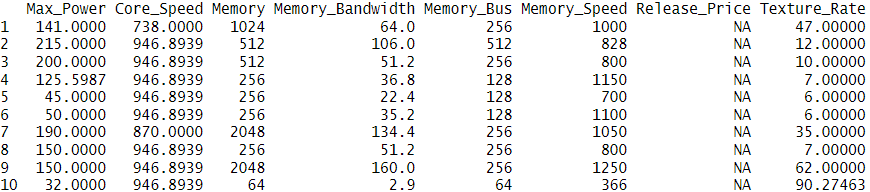
\includegraphics[width=\linewidth]{4. GPU/Console/console5.png}
                    \caption{Thống kê dữ liệu bị khuyết ở các cột}
                \end{figure}
                \vspace{-20pt}
                \item \fontsize{13pt}{15pt}\selectfont Xóa dữ các dòng bị khuyết của biến Release\_Price.
\begin{mybox}{R Code}
    \begin{lstlisting}[language={R}] 
    all_gpus_news_clean <- na.omit(all_gpus_news)
    head(all_gpus_news_clean)
    \end{lstlisting}
\end{mybox}
                \begin{figure}[H]
                    \vspace{-7pt}
                    \centering
                    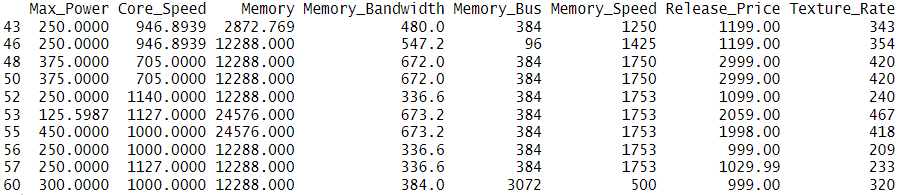
\includegraphics[width=\linewidth]{4. GPU/Console/console6.png}
                    \caption{Dữ liệu sau khi lọc bỏ các hàng bị khuyết của biến Release\_Price}
                \end{figure}
                \vspace{-20pt}
                \item \fontsize{13pt}{15pt}\selectfont Đánh lại số thứ tự các dòng dữ liệu.
\begin{mybox}{R Code}
    \begin{lstlisting}[language={R}] 
    rownames(all_gpus_news_clean) <- NULL
    head(all_gpus_news_clean)
    \end{lstlisting}
\end{mybox}
                \begin{figure}[H]
                    \vspace{-7pt}
                    \centering
                    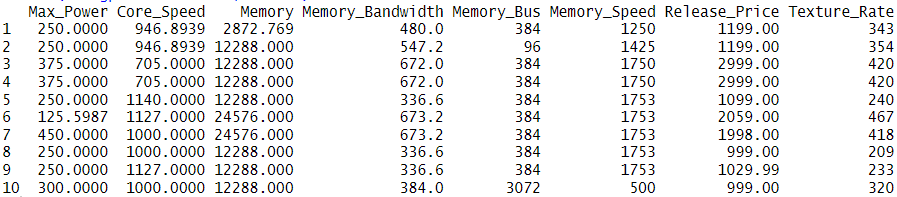
\includegraphics[width=\linewidth]{4. GPU/Console/console7.png}
                    \caption{Dữ liệu sau khi đánh lại số thứ tự}
                \end{figure}
            \end{itemize}

\newpage
    \begin{center}
        \section*{THỐNG KÊ TẢ GPU}
    \end{center}
    \addcontentsline{toc}{section}{4. Thống kê tả GPU}
        \subsection*{4.1 Scatter plots}
        \addcontentsline{toc}{subsection}{4.1 Scatter plots}
            \begin{figure}[!h]
                \centering
                \includesvg[scale=.3]{4. GPU/Rplot/Rplot03.svg}
                \includesvg[scale=.3]{4. GPU/Rplot/Rplot04.svg}
                \includesvg[scale=.3]{4. GPU/Rplot/Rplot05.svg}
                \includesvg[scale=.3]{4. GPU/Rplot/Rplot06.svg}
                \includesvg[scale=.3]{4. GPU/Rplot/Rplot07.svg}
                \includesvg[scale=.3]{4. GPU/Rplot/Rplot08.svg}
                \includesvg[scale=.3]{4. GPU/Rplot/Rplot09.svg}
                \caption{Biểu đồ phân tán của 7 biến đối với biến Release\_Price}
            \end{figure}
            
\newpage
        \hspace{1pt}
        \fontsize{13pt}{15pt}\selectfont \textbf{Nhận xét}: Dựa vào các biểu đồ, giá trị “Release\_Price” dao động trong khoảng 49\$ tới 15\$. Tuy nhiên, ta chỉ có thể vẽ đường hồi quy cho các biến “Texture\_Rate”, “Memory\_Bandwidth”. Nghĩa là, “Release\_Price” có mối quan hệ tuyến tính mạnh với các biến này. Vì thế, ta có thể kết luận rằng mối quan hệ giữa các biến này là mối quan hệ tuyến tính giữa các biến độc lập là thuận và tương đối mạnh khi mà ta có thể vẽ được đường thẳng hồi quy với xu hướng đi lên.
            
        \subsection*{4.2 Histogram}
        \addcontentsline{toc}{subsection}{4.2 Histogram}
            \gachdau
            Nhóm đã tiến hành vẽ biểu đồ tần suất (Histogram) nhằm biểu thị mức độ phân phối của bộ dữ liệu được cung cấp.
            \begin{figure}[H]
                \vspace{3pt}
                \centering
                \includesvg[width=\linewidth]{4. GPU/Rplot/Rplot02.svg}
                \caption{Biểu đồ cột của 8 biến}
            \end{figure}
            \vspace{-15pt}
            \hspace{1pt}
            \fontsize{13pt}{15pt}\selectfont \textbf{Nhận xét}: Dựa trên các Histogram, ta có thể thấy rằng giá trị của biến “Release\_Price” chủ yếu giao động ở mức 0\$ đến 500\$ và tập trung chủ yếu trong khoảng 50\$ đến 250\$. Giá trị có số lượng ít nhất là trong khoảng 800\$ đến 900\$.

\newpage
        \subsection*{4.3 Boxplot}
        \addcontentsline{toc}{subsection}{4.3 Boxplot}
            \begin{figure}[H]
                \vspace{-20pt}
                \centering
                \includesvg[width=0.65\linewidth]{4. GPU/Rplot/boxplot1.svg}
                \caption{Biểu đồ boxplot của 2 biến \textcolor{blue}{Max\_Power} và \textcolor{blue}{Core\_Speed}.}
            \end{figure}
            \vspace{-29pt}
            \begin{figure}[H]
                \centering
                \includesvg[width=0.65\linewidth]{4. GPU/Rplot/boxplot2.svg}
                \caption{Biểu đồ boxplot của 2 biến \textcolor{blue}{Memory} và \textcolor{blue}{Memory\_Bandwidth}.}
            \end{figure}
            \vspace{-29pt}
            \begin{figure}[H]
                \centering
                \includesvg[width=0.65\linewidth]{4. GPU/Rplot/boxplot3.svg}
                \caption{Biểu đồ boxplot của 2 biến \textcolor{blue}{Memory\_Bus}  và \textcolor{blue}{Memory\_Speed}.}
            \end{figure}
            \vspace{-29pt}
            \begin{figure}[H]
                \centering
                \includesvg[width=0.65\linewidth]{4. GPU/Rplot/boxplot4.svg}
                \caption{Biểu đồ boxplot của 2 biến \textcolor{blue}{Release\_Price} và \textcolor{blue}{Textur\_Rate}.}
            \end{figure}

\newpage
            \hspace{1pt}
            \fontsize{13pt}{15pt}\selectfont \textbf{Nhận xét}: Nhìn chung, có nhiều điểm ngoại lai nên khiến ta không thể nhìn rõ điểm phân phối, vậy nên chúng ta cần xử lí và vẽ lại đồ thị”.\\
            \gachdau
            \fontsize{13pt}{15pt}\selectfont  Các điểm ngoại lệ có thể được xử lý bằng cách clip về giá trị cực tiểu và cực đại của Box plot. Tức là khi một giá trị quá lớn hoặc quá nhỏ, ta đưa nó về giá trị lớn nhất/nhỏ nhất được coi là những điểm bình thường.
\begin{mybox}{R Code}
\begin{lstlisting}[language={R}] 
    find_boxplot_boundaries<-function(col,whisker_coeff=1.5){
      Q1 <- quantile(col, 0.25)
      Q3 <- quantile(col, 0.75)
      IQR <- Q3 - Q1
      lower <- Q1 - whisker_coeff * IQR
      upper <- Q3 + whisker_coeff * IQR
      return(list(lower = lower, upper = upper))
      }
      
    BoxplotOutlierClipper<-function(whisker_coeff = 1.5, X){
      boundaries <- find_boxplot_boundaries(X, whisker_coeff)
      clipped_X <- pmax(pmin(X, boundaries$upper), boundaries$lower)
      return(clipped_X)
      }
\end{lstlisting}
\end{mybox}
            \hspace{1pt}
            \fontsize{13pt}{15pt}\selectfont Áp dụng lại vào dữ liệu của cột của các biến ta có histogram và boxplot mới như sau:
            \vspace{-10pt}
            \begin{figure}[H]
                \centering
                \includesvg[width=0.49\linewidth]{4. GPU/Rplot/max_power.svg}
                \includesvg[width=0.49\linewidth]{4. GPU/Rplot/Core_Speed.svg}
                \includesvg[width=0.49\linewidth]{4. GPU/Rplot/memory.svg}
                \includesvg[width=0.49\linewidth]{4. GPU/Rplot/Memory_Bandwidth.svg}
                \includesvg[width=0.49\linewidth]{4. GPU/Rplot/Memory_bus.svg}
                \includesvg[width=0.49\linewidth]{4. GPU/Rplot/Memory_Speed.svg}
                \includesvg[width=0.49\linewidth]{4. GPU/Rplot/Release_Price.svg}
                \includesvg[width=0.49\linewidth]{4. GPU/Rplot/Texture_Rate.svg}
                \caption{Biểu đồ histogram và boxplot của 8 biến sau xử lí các giá trị ngoại lai}
            \end{figure}
            \vspace{-15pt}
            \hspace{1pt}
            \fontsize{13pt}{15pt}\selectfont \textbf{Nhận xét}: Sau khi xử lí dữ liệu theo cực tiểu và cực đại của box plot, ta thấy rằng dữ liệu đỡ bị lệch đi. Box plot cũng cho thấy không còn điểm dữ liệu ngoại lệ nào. Các biều đồ histogram hầu như không thay đổi quá lớn so với lúc chưa xử lí các giá trị ngoại lai và ta có thể nhìn rõ sự phân bố của các biến, qua đó có thể thấy rằng giá của GPU trải dài và đa dạng. Các biểu đồ box plot hầu như lệch trái cũng thể hiện giá của GPU thường ở mức trung bình, thấp tiếp cận được với đại đa số khách hàng.

\newpage
        \subsection*{4.4 Tính giá trị thống kê mô tả}
        \addcontentsline{toc}{subsection}{4.4 Tính giá trị thống kê mô tả}
            \gachdau
            Tính các giá trị thống kê mô tả gồm: trung bình, trung vị, độ lệch chuẩn, giá trị lớn nhất và giá trị nhỏ nhất, xuẩt kết quả dưới dạng bảng ta thu được như sau:
            
\begin{mybox}{R Code}
\begin{lstlisting}[language={R}] 
 thongkemota <- data.frame(
  cbind(
    apply(all_gpus_news_clean, MARGIN=2, min),
    apply(all_gpus_news_clean, MARGIN=2, sd),
    apply(all_gpus_news_clean, MARGIN=2, mean),
    apply(all_gpus_news_clean, MARGIN=2, median),
    apply(all_gpus_news_clean, MARGIN=2, max)
  )
 )

 colnames(thongkemota) <- c("GTNN(min)", "Do lech chuan (sd)", "Trung binh (mean)", "Trung vi (median)", "GTLN (max)")
 head(thongkemota)
\end{lstlisting}
\end{mybox}
            
            \begin{table}[htbp]
              \centering
              \scriptsize
              \caption{Bảng giá trị thống kê mô tả các của các biến}
              \begin{tabular}{lrrrrr}
                \toprule
                & GTNN(min) & Độ lệch chuẩn (sd) & Trung bình (mean) & Trung vị (median) & GTLN(max) \\
                \midrule
                Max\_Power          & 18.0000     & 70.31991          & 153.6982            & 150.0    & 310.000 \\
                Core\_Speed        & 604.7348    & 229.16461         & 1072.8082           & 1024.5   & 1517.159 \\
                Memory            & 512.0000    & 3238.46282        & 4724.6154           & 4096.0   & 17408.000 \\
                Memory\_Bandwidth   & 12.8000     & 109.80099         & 208.1493            & 192.3    & 471.850 \\
                Memory\_Bus         & 64.0000     & 98.51261          & 224.8251            & 256.0    & 448.000 \\
                Memory\_Speed      & 808.0000    & 366.05475         & 1583.0270           & 1750.0   & 2127.000 \\
                \bottomrule
              \end{tabular}
            \end{table}
            
\newpage
    \begin{center}
        \section*{THỐNG KÊ SUY DIỄN GPU}
    \end{center}
    \addcontentsline{toc}{section}{5. Thống kê suy diễn GPU}
        \subsection*{5.1 Xây dựng mô hình hồi quy tuyến tính}
        \addcontentsline{toc}{subsection}{5.1 Xây dựng mô hình hồi quy tuyến tính}
            \gachdau
            Xét mô hình hổi quy gồm:
            \begin{itemize}[leftmargin=3.5em, itemsep=-1.5em, parsep=1.6em]
                \vspace{-6pt}
                \item \fontsize{13pt}{15pt}\selectfont Biến phụ thuộc: \textcolor{blue}{Release\_Price}.
                \item \fontsize{13pt}{15pt}\selectfont Biến độc lập: \textcolor{blue}{Max\_Power}, \textcolor{blue}{Core\_Speed}, Memory, \textcolor{blue}{Memory\_Bandwidth}, \textcolor{blue}{Memory\_Bus}, \textcolor{blue}{Memory\_Speed}, \textcolor{blue}{Texture\_Rate}.
            \end{itemize}
            \vspace{-7pt}
            \gachdau
            Ta có mô hình:
            \vspace{-18pt}
            \begin{align*}
                Release\_Price = \beta_0 + \beta_1 \cdot Max\_Power + \beta_2 \cdot Core\_Speed + \beta_3 \cdot Memory + \beta_4 \cdot \\
                Memory\_Bandwidth + \beta_5 \cdot Memory\_Bus + \beta_6 \cdot Memory\_Speed + \beta_7 \cdot Texture\_Rate
            \end{align*}
            \begin{figure}[H]
                \vspace{-18pt}
                \centering
                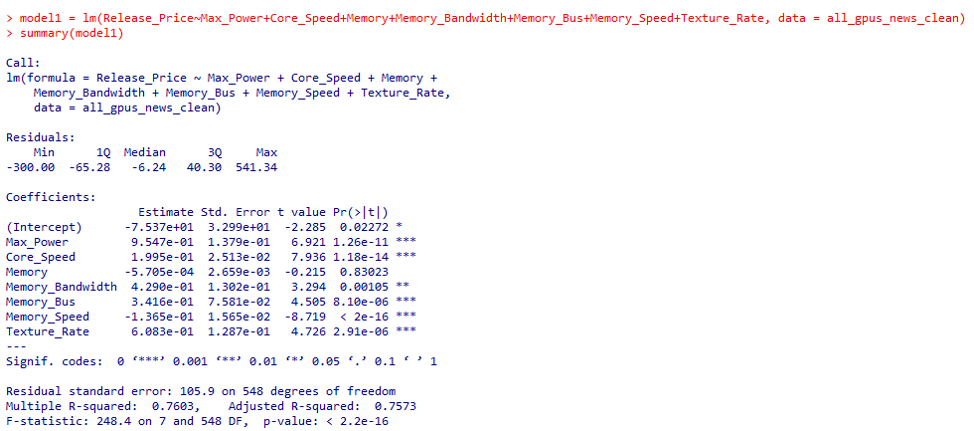
\includegraphics[width=\linewidth]{4. GPU/Thống kê suy diễn/model1.png}
                \caption{Ước lượng hệ số $\beta_i$ $(0 \leq i \leq 7)$ dựa trên tệp all\_gpus\_news\_clean (model1)}
            \end{figure}
            \vspace{-16pt}
            \hspace{1pt}
            Do $P_r (> |t|)$ của tất cả các biến trừ Memory và hệ số tự do đều bé hơn mức ý nghĩa 0.05, nên ta bác bỏ giả thuyết $H_0$ của các biến trừ Memory. Tuy nhiên, do chưa đủ căn cứ để khẳng định giả thuyết $H_0$ đối với Memory, nhóm quyết định xây dựng thêm một mô hình model2 bằng cách loại bớt biến Memory khỏi mô hình model1.

\newpage
            \begin{figure}[H]
                \vspace{-5pt}
                \centering
                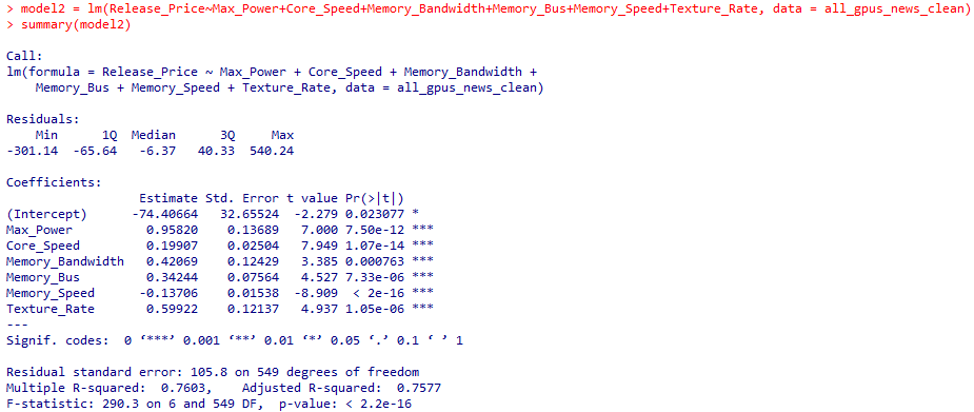
\includegraphics[width=\linewidth]{4. GPU/Thống kê suy diễn/model2.png}
                \caption{mô hình model2 loại bớt biến Memory khỏi mô hình model1}
            \end{figure}
            \vspace{-16pt}
            \hspace{1pt}
            Tiến hành so sánh hai mô hình với giả thuyết:
            \begin{itemize}[leftmargin=3.5em, itemsep=-1.5em, parsep=1.6em]
                \vspace{-6pt}
                \item \fontsize{13pt}{15pt}\selectfont $H_0$: Hai mô hình có độ hiệu quả như nhau.
                \item \fontsize{13pt}{15pt}\selectfont $H_1$: Hai mô hình có độ hiệu quả khác nhau.
            \end{itemize}
            \vspace{-7pt}
            \gachdau
            Phân tích phương sai ANOVA:
            \begin{figure}[H]
                \vspace{-5pt}
                \centering
                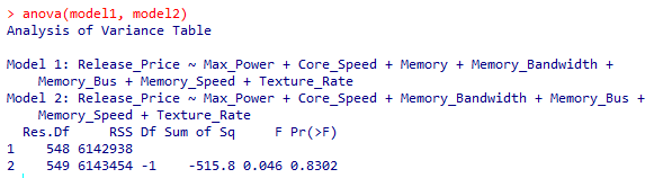
\includegraphics[width=\linewidth]{4. GPU/Thống kê suy diễn/ANOVA.png}
                \caption{Phương sai ANOVA}
            \end{figure}
            \vspace{-16pt}
            \hspace{1pt}
            Vì $P_r (> T) = 0.8302 > 0.05$ nên giả thuyết $H_0$ là phù hợp. Do cả hai mô hình đều có độ hiệu quả như nhau, nên việc loại bỏ biến Memory không gây ảnh hưởng tới mô hình ta đã xây dựng, vì vậy nhóm quyết định chọn mô hình model2 là mô hình phù hợp hơn.\\
            \gachdau
            Như vậy đường thẳng hồi quy ước lượng được cho bởi phương trình:
            \vspace{-18pt}
            \begin{align*}
                Release\_Price = -74.40664 + 0.95820 \cdot Max\_Power + 0.19907 \cdot Core\_Speed -\\
                0.42069 \cdot Memory\_Bandwidth + 0.34244 \cdot Memory\_Bus -\\
                0.13706 \cdot Memory\_Speed + 0.59922 \cdot Texture\_Rate
            \end{align*}
\newpage
            \hspace{1pt}
            Ngoài ra ta cũng thấy được hệ số $R^2$ hiệu chỉnh là 0.7577 cho thấy đến 75.77\% sự biến thiên trong giá máy tính được giải thích bằng các biến độc lập, 24.23\% còn lại có thể do sai số hoặc các biến độc lập khác chưa được đưa vào mô hình.
            \gachdau
            Cuối cùng, ta đi kiểm tra tính phù hợp của mô hình vừa thu được thông qua các đồ thị:
            \begin{figure}[H]
                \vspace{-6pt}
                \centering
                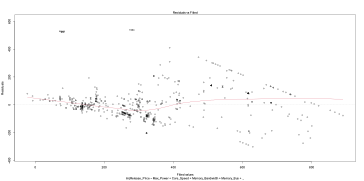
\includegraphics[width=0.44\textwidth]{4. GPU/Thống kê suy diễn/Rplot1.png}
                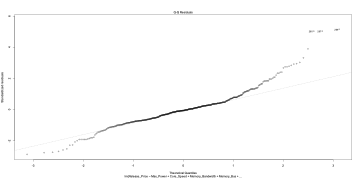
\includegraphics[width=0.44\textwidth]{4. GPU/Thống kê suy diễn/Rplot2.png}
                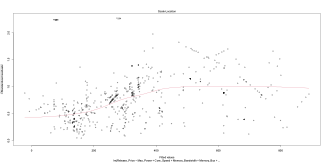
\includegraphics[width=0.44\textwidth]{4. GPU/Thống kê suy diễn/Rplot3.png}
                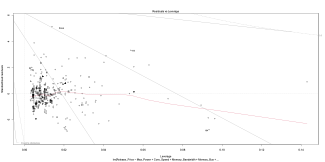
\includegraphics[width=0.44\textwidth]{4. GPU/Thống kê suy diễn/Rplot4.png}
            \end{figure}
            \vspace{-5pt}
            \hspace{1pt}
            \fontsize{13pt}{15pt}\selectfont \textbf{Nhận xét}: \begin{itemize}[leftmargin=3.5em, itemsep=-1.5em, parsep=1.6em]
                \vspace{-6pt}
                \item \fontsize{13pt}{15pt}\selectfont Đồ thị thứ 1 (Residuals vs Fitted) vẽ các giá trị sai số so với dự báo, dùng để kiểm tra giả thiết tuyến tính của dữ liệu và giả thiết sai số có kỳ vọng bằng 0. Đường màu đỏ gần với đường thẳng $y = 0$, tuy có sai lệch nhưng vẫn trong khoảng chấp nhận được, chứng tỏ bộ dữ liệu có tính tuyến tính, và giả thiết sai số có kỳ vọng bằng 0 thỏa mãn.
                \item \fontsize{13pt}{15pt}\selectfont Đồ thị thứ 2 (Q-Q Residuals) vẽ sai số được chuẩn hóa, dùng để kiểm tra giả thiết sai số có phân phối chuẩn. Các điểm trên đồ thị được phân bố theo đường thẳng màu đỏ, chỉ sai lệch ở hai đầu nên giả thiết sai số có phân phối chuẩn thỏa mãn.
                \item \fontsize{13pt}{15pt}\selectfont Đồ thị thứ 3 (Scale – Location) vẽ căn bậc hai của sai số được chuẩn hóa dùng để kiểm tra giả định phương sai của sai số là hằng số. Các điểm phân tán một cách ngẫu nhiên, không tập trung nhiều quanh đường màu đỏ nên giả định về phương sai của sai số là hằng số được thỏa mãn.
                \item \fontsize{13pt}{15pt}\selectfont Đồ thị thứ 4 (Residuals vs Leverage) dùng để xác định các điểm có ảnh hưởng cao. Các điểm đó là 184, 265 và 183.
            \end{itemize}

\newpage
        \subsection*{5.2 Dự báo cho giá GPU}
        \addcontentsline{toc}{subsection}{5.2 Dự báo cho giá GPU}
            \begin{itemize}
                \vspace{-6pt}
                \item \fontsize{13pt}{15pt}\selectfont Dựa trên mô hình hồi quy đã xây dựng, thử dự báo giá một GPU có: $Max\_Power = 141W$, $Core\_Speed = 738MHz$, $Memory = 1024MB$, $Memory\_Bandwidth = 64GB/sec$, $Memory\_Bus = 256bit$, $Memory\_Speed = 1000MHz$, $Texture\_Rate = 47Gtexel/s$.
                \begin{figure}[H]
                    \centering
                    \includegraphics[width=0.9\linewidth]{4. GPU/Thống kê suy diễn/Dự báo giá.png}
                \end{figure}
                \item \fontsize{13pt}{15pt}\selectfont Giá dự báo 213.3062 với khoảng tin cậy so với giá trị dự báo $(190.1539, 236.4586)$.
            \end{itemize}

\newpage
    \begin{center}
        \section*{THẢO LUẬN VÀ MỞ RỘNG}
    \end{center}
    \addcontentsline{toc}{section}{6. Thảo luận và mở rộng}
        \vspace{-1pt}
        \subsection*{6.1 Ưu điểm}
        \addcontentsline{toc}{subsection}{6.1 Ưu điểm}
            \vspace{-4pt}
            \gachdau
            Hồi quy tuyến tính bội giúp phân tích đồng thời tác động của nhiều biến độc lập lên một biến phụ thuộc. Điều này giúp chúng ta xác định được tầm quan trọng tương đối của từng biến độc lập trong việc dự đoán biến phụ thuộc.\\
            \gachdau
            Bằng cách sử dụng 6 yếu tố chính tác động đến biến phụ thuộc “Release\_Price”, chúng ta đã có thể dự đoán giá bán ra của các GPU.\\
            \gachdau
            Phân tích phương sai ANOVA cho phép kiểm định sự khác biệt giữa các nhóm của biến phụ thuộc, giúp hiểu rõ hơn về ảnh hưởng của các yếu tố. Đồng thời, phương pháp này giúp phân tích sự biến thiên của dữ liệu và xác định xem có yếu tố nào ảnh hưởng đáng kể đến giá bán GPU hay không.

        \vspace{-7pt}
        \subsection*{6.2 Hạn chế}
        \addcontentsline{toc}{subsection}{6.2 Hạn chế}
            \vspace{-4pt}
            \gachdau
            Chỉ có thể sử dụng cho kiểu dữ liệu tuyến tính.\\
            \gachdau
            Để mô hình hoạt động hiệu quả, cần phải loại bỏ các điểm ngoại lai là những giá trị quan trắc có sự khác biệt đáng kể so với các giá trị quan trắc khác trong bộ dữ liệu vì chúng có thể làm sai lệch mối quan hệ giữa biến dự đoán và biến phụ thuộc và dẫn đến dự đoán không chính xác.\\
            \gachdau
            Phân tích phương sai ANOVA chỉ mô tả sự khác biệt giữa các nhóm mà không xác định được mối quan hệ nhân quả giữa các biến.

        \vspace{-7pt}
        \subsection*{6.3 Mở rộng}
        \addcontentsline{toc}{subsection}{6.3 Mở rộng}
            \vspace{-4pt}
            \gachdau
            Nguồn dữ liệu cần được thu thập và mở rộng để có nguồn dữ liệu toàn diện hơn, nhiều đặc điểm nghiên cứu hơn. Từ đó, đưa ra dự đoán một cách khách quan hơn, tăng tỉ lệ chính xác cho dự đoán.\\
            \gachdau
            Bên cạnh đó, để mang lại hiệu quả dự đoán tốt nhất thì các phương pháp dự đoán cũng cần sử dụng một cách linh hoạt. Chúng ta có thể sự dụng một số phương pháp khác như: Mô hình hồi quy tuyến tính, Mô hình hồi quy phi tuyến, Mô hình hồi quy lựa chọn, Mô hình hồi quy đa cấp,...\\
            \gachdau
            Tuy nhiên, hạn chế về mặt thời gian và kiến thức nên chúng em chỉ sử dụng Mô hình hồi quy bội để dự đoán kết quả. 

\newpage
    \begin{center}
        \section*{NGUỒN DỮ LIỆU VÀ NGUỒN CODE}
    \end{center}
    \addcontentsline{toc}{section}{7. Nguồn dữ liệu và nguồn code}
        \subsection*{7.1 Nguồn dữ liệu}
        \addcontentsline{toc}{subsection}{7.1 Nguồn dữ liệu}
            \url{https://www.kaggle.com/datasets/iliassekkaf/computerparts}

        \subsection*{7.2 Nguồn code}
        \addcontentsline{toc}{subsection}{7.2 Nguồn code}
            \href{https://drive.google.com/drive/folders/1O10XfZgub6dYam8kqlon-0puwhi4C7Ef?usp=sharing}{\nolinkurl{https://drive.google.com/drive/folders/1O10XfZgub6dYam8kql}} \\
            \href{https://drive.google.com/drive/folders/1O10XfZgub6dYam8kqlon-0puwhi4C7Ef?usp=sharing}{\nolinkurl{on-0puwhi4C7Ef?usp=sharing}}       
            
\newpage
    \addcontentsline{toc}{section}{8. Tài liệu tham khảo}
    \begin{center}
        \begin{thebibliography}{99}
            \item Nguyễn Kiều Dung, \textit{Bài giảng Xác suất Thống Kê}.
            \item Nguyễn Tiến Dũng (chủ biên), Nguyễn Đình Huy, 2019, \textit{Xác suất - Thống kê \& Phân tích số liệu}.
            \item Hoàng Văn Hà, \textit{Bài giảng Xác suất Thống Kê}.
            \item Lê Hồng Thái, \textit{Phương pháp tính toán và đánh giá độ tin cậy trong hệ thống điện}.
            \item Nguyễn Đình Thắng, \textit{Giáo trình Vật liệu điện}.
            \item George C.Runner.Hoboken, Douglas C.Montgomery, 2007, \textit{Applied Statistic and Probability for Engineers}, NJ: Wiley.
            \item David M. Rocke, 2020, Geoffrey J. Thompson, \textit{Applied Statistics with R}, NY: Springer.
        \end{thebibliography}
    \end{center}
\end{document}
